%!TEX root = ../swiatlow_thesis.tex
\label{chapter:jet-reconstruction}


Jet reconstruction in ATLAS makes use of the algorithms described in~\ref{chapter:jets-and-substructure} to create 4-vectors and other observables usable for physics analysis. As previously discussed, a wide variety of algorithms, with various uses and benefits compared to others, are available in the literature. ATLAS most typically makes use of:

\begin{enumerate}
	\item \antikt with $R = 0.4$
	\item \antikt with $R = 0.6$
	\item \antikt with $R = 1.0$, using Trimming with $\Rsub = 0.3$, $\fcut = 5\%$
\end{enumerate}
%
Some analyses also make use of various \CAFat jets, with various forms of split-filtering or reclustered-mass-drop filtering \editnote{Cite these.}. The analyses presented in in this thesis utilize the first and third algorithms, and most of the discussion that follows will focus on various aspects of the reconstruction of these jets.

There are many more aspects to creating a jet than just choosing an algorithm, and this chapter covers the various aspects of jet reconstruction from inputs to calibrations and flavor identification. Note that while the jet reconstruction and calibration procedure has evolved significantly since the start of data-taking, some aspects have not changed very much. While all the procedures described follow the latest developments in ATLAS, some of the demonstrative figures may use older data if that particular procedure has not changed.

\section{Jet Inputs}


One of the most important decisions in constructing a jet is the decision of what to actually input to the jet algorithm-- i.e., the choice of what to cluster. Several inputs are available, summarized in Figure~\ref{fig:jet-reconstruction:making-jets}. 

%%%%%%%%%%%%%%%%

\begin{figure}
\centering
\includegraphics[width=0.7\textwidth]{making-jets.pdf}
\label{fig:jet-reconstruction:making-jets}
\caption{A diagram showing the various forms of jet inputs, and the different types of jets they are used to make.}
\end{figure}

%%%%%%%%%%%%%%%% 

Jets constructed from the simulated particles from a Monte Carlo generator are called \textit{truth jets}: these are primarily used to study the performance of algorithms without the effect of the detector, and to calibrate and define the resolution of other classes of jets. 

Jets can also be constructed from tracks, the outputs of pattern recognition algorithms performed on the hits in the Inner Detector, which correspond to the trajectories of charged particles. These \textit{track jets} are mostly used for validation: they provide a completely independent measurement of a jet from the calorimeter, and while they miss the neutral third of particles, the increased angular precision of tracking can result in complementary information to the calorimeter measurement. \editnote{Cite Seth's thesis, substructure paper?} 

Finally, and most importantly, jets can be formed from energy deposits left in the calorimeter, and these are called \textit{calorimeter jets}. Historically, ATLAS went through many different options for reducing the calorimeter information to a more manageable form for input to jet algorithms-- algorithms such as Global Cell Weighting, Noise Suppressed Towers, and simple projective towers were all eventually disfavored compared to the topo-clustering algorithm described in Section~\ref{jet-reconstruction:jet-inputs:topoclustering}. Calorimeter measurements all share several properties: they provide a measurement of the total energy of the parton shower, produced in both neutral and charged particles. This measurement of the jet (after relevant calibrations are applied) is at approximately the same scale as the quark which initiated it: for example, the invariant mass of the leading non-$b$-tagged jets in semi-leptonic $t\bar{t}$ peaks at the value of the mass of the $W$-boson, $m_{W} = 80$~GeV. Calorimeter jets can thus be used as 4-vectors in the same way that other detector objects-- electrons, photons, etc.-- are used (though of course there is more information in the structure of these jets, which analyses in this thesis do exploit).  \editnote{Add a few citations}

One alternative to separate tracking and calorimeter reconstructions of jets is to use a ``particle flow'' algorithm to combine the measurements from the separate detectors into coherent particle candidates which an be used as inputs to jet algorithms. Such algorithms exploit the fact that charged particles are much more accurately measured (up to some crossing point determined by the strength of the magnetic field) by tracking systems rather than calorimeter systems. Typically, tracks are extrapolated to the calorimeter and matched to energy deposits there; these matched deposits are then subtracted from the calorimeter, as the energy is already accounted for by the tracker. Unmatched energy deposits are assumed to have been created by photons or neutral hadrons, and remain in the list of inputs. Thus, the best features of tracker measurements (accurate energy resolution, and very good angular precision) and calorimeter measurements (capability of measuring neutral particles, good energy resolution at high energies) are combined. The CMS detector is particularly well suited to such reconstruction: the calorimeters are inside the 3.8 T magnetic field (nearly two times stronger than ATLAS), so energy deposits are more widely separated and track-to-calorimeter matching is less ambiguous. Since two thirds of the particles in the jet are reconstructed with tracks instead of calorimeter measurements, the reduced performance of the CMS hadronic calorimeters is also less important. However, as ATLAS has a weaker (and smaller, spatially) magnetic field, and compartively stronger hadronic calorimeters, the improvement from this approached is much diminished and ATLAS has thus far not used the particle flow algorithm for analyses. \editnote{Cite this as well}

The following subsections describe some details of the topoclustering and tracking algorithms which form the inputs to the jet algorithms in ATLAS. The design decisions in these algorithms-- and the strong performance they achieve in the face of difficult operating conditions-- are critical for the final results of hadronic analyses on ATLAS.

\subsection{Topoclustering}
\label{jet-reconstruction:jet-inputs:topoclustering}

Energy measurements in the calorimeter are done at the \textit{cell} level, the smallest read-out unit in the calorimeter. Cells, however, are not particularly well suited for constructing jets for a number of reasons: they are very noisy, they are very sensitive to pileup, one particle can leave energy in many different cells,  there are too many for the $\mathrm{O}( n \log n)$ jet clustering algorithms to efficiently cluster, etc. Topo-clustering is one algorithm, out of many historical altenatives, to efficiently reduce cells to a more manageable, less noisy object~\cite{JES2010,JES2011}.

Topo-clusters, short for ``three dimensional topological clusters,'' sum the scalar energy measured in adjacent cells joined by the clustering algorithm. The clustering is based on the principle of measured energy significance in each cell, defined as $E/\sigma_{\mathrm{noise}}$ where $\sigma_\mathrm{noise}$ is defined as $\sigma_\mathrm{noise} = \sigma^\mathrm{electronic}_\mathrm{noise}~\oplus~\sigma^\mathrm{pileup}_\mathrm{noise}$~\cite{JES2010,JES2011}. The first term corresponds to the expected electronics noise from the detector readout in that cell; the second term corresponds to the expected variation in the energy measurement caused by pileup in that cell. $\sigma^\mathrm{pileup}_\mathrm{noise}$ is set to a value of the expected $\mu$, which was $30$ during 2012 conditions. For most of the detector $\eta$, $\sigma^\mathrm{electronic}_\mathrm{noise} \approx \sigma^\mathrm{pileup}_\mathrm{noise}$, except in the forward region where $\sigma^\mathrm{pileup}_\mathrm{noise}$ is much larger due to the large forward flux (and larger cell size). Figure~\ref{fig:jet-reconstruction:jet-inputs:topoclustering-noise} shows the different total noise expected in each of 2010, 2011, and 2012; the rising values indicate the greater expected presence of pileup.

%%%%%%%%%%%%%%%%%%%%%

\begin{figure}
\centering
\subfigure[2010]{\includegraphics[width=0.45\textwidth]{topo_2010}}
\subfigure[2011]{\includegraphics[width=0.45\textwidth]{topo_2011}}

\subfigure[2012]{\includegraphics[width=0.45\textwidth]{topo_2012}}
\label{fig:jet-reconstruction:jet-inputs:topoclustering-noise}
\caption{Total expected noise, $\sigma_\mathrm{noise} = \sigma^\mathrm{electronic}_\mathrm{noise}~\oplus~\sigma^\mathrm{pileup}_\mathrm{noise}$, in each year of detector operations, for various subdetectors, as a function of $\eta$. The higher levels in 2011 and 2012 compared to 2012 indicate the changing pileup noise threshold.}
\end{figure}

%%%%%%%%%%%%%%%%%%%%%

Each cell thus has an energy significance $\zeta = E / \sigma_\mathrm{noise}$~\cite{JES2010,JES2011}. Topo-clusters are \textit{seeded} by cells with a significance of $S$ (typically 4) or greater. All cells surrounding the seed cell (either directly neighboring if the cells are in the same layer, or overlapping in $\eta/\phi$ if in different layers) with significance $N$ (typically 2) or greater are then joined to the seed. This \textit{growth} stage continues iteratively for all adjoining cells with $\zeta > N$. As a last step, all cells with significance larger than $P$ (typically 0) adjoining the growth-stage cells are also joined to the cluster: this is referred to as the \textit{boundary}. Finally, a splitting algorithm can split clusters into two at a boundary between two local maxima. Typically, clusters are expected to be produced approximately once by each particle in the calorimeter, though multiple clusters can be created depending on the way the particle interacts. Note that all energies measured are absolute: negative energy cells are allowed to join topo-clusters. Negative energy cells originate from the pulse shaping of the LAr calorimeter, and these negative fluctuations (many caused by pileup) are expected to partly cancel the positive fluctuations caused by pileup. The noise-suppression aspect of topo-clustering significantly improves the performance of the calorimeter by removing isolated fluctuations due to electronics noise and pileup, though particularly large fluctuations can still survive the seeding requirement. Figure~\ref{fig:jet-reconstruction:jet-inputs:topoclustering-display} shows cells at the various stages of the topo-clustering, in one layer of the calorimeter.

%%%%%%%%%%%%%%%%%%%%%

\begin{figure}
\centering
\subfigure[Seed cells]{\includegraphics[width=0.45\textwidth]{FCal_evtdisplay_2sig.pdf}}
\subfigure[Growth cells]{\includegraphics[width=0.45\textwidth]{FCal_evtdisplay_4sig.pdf}}

\subfigure[All cells]{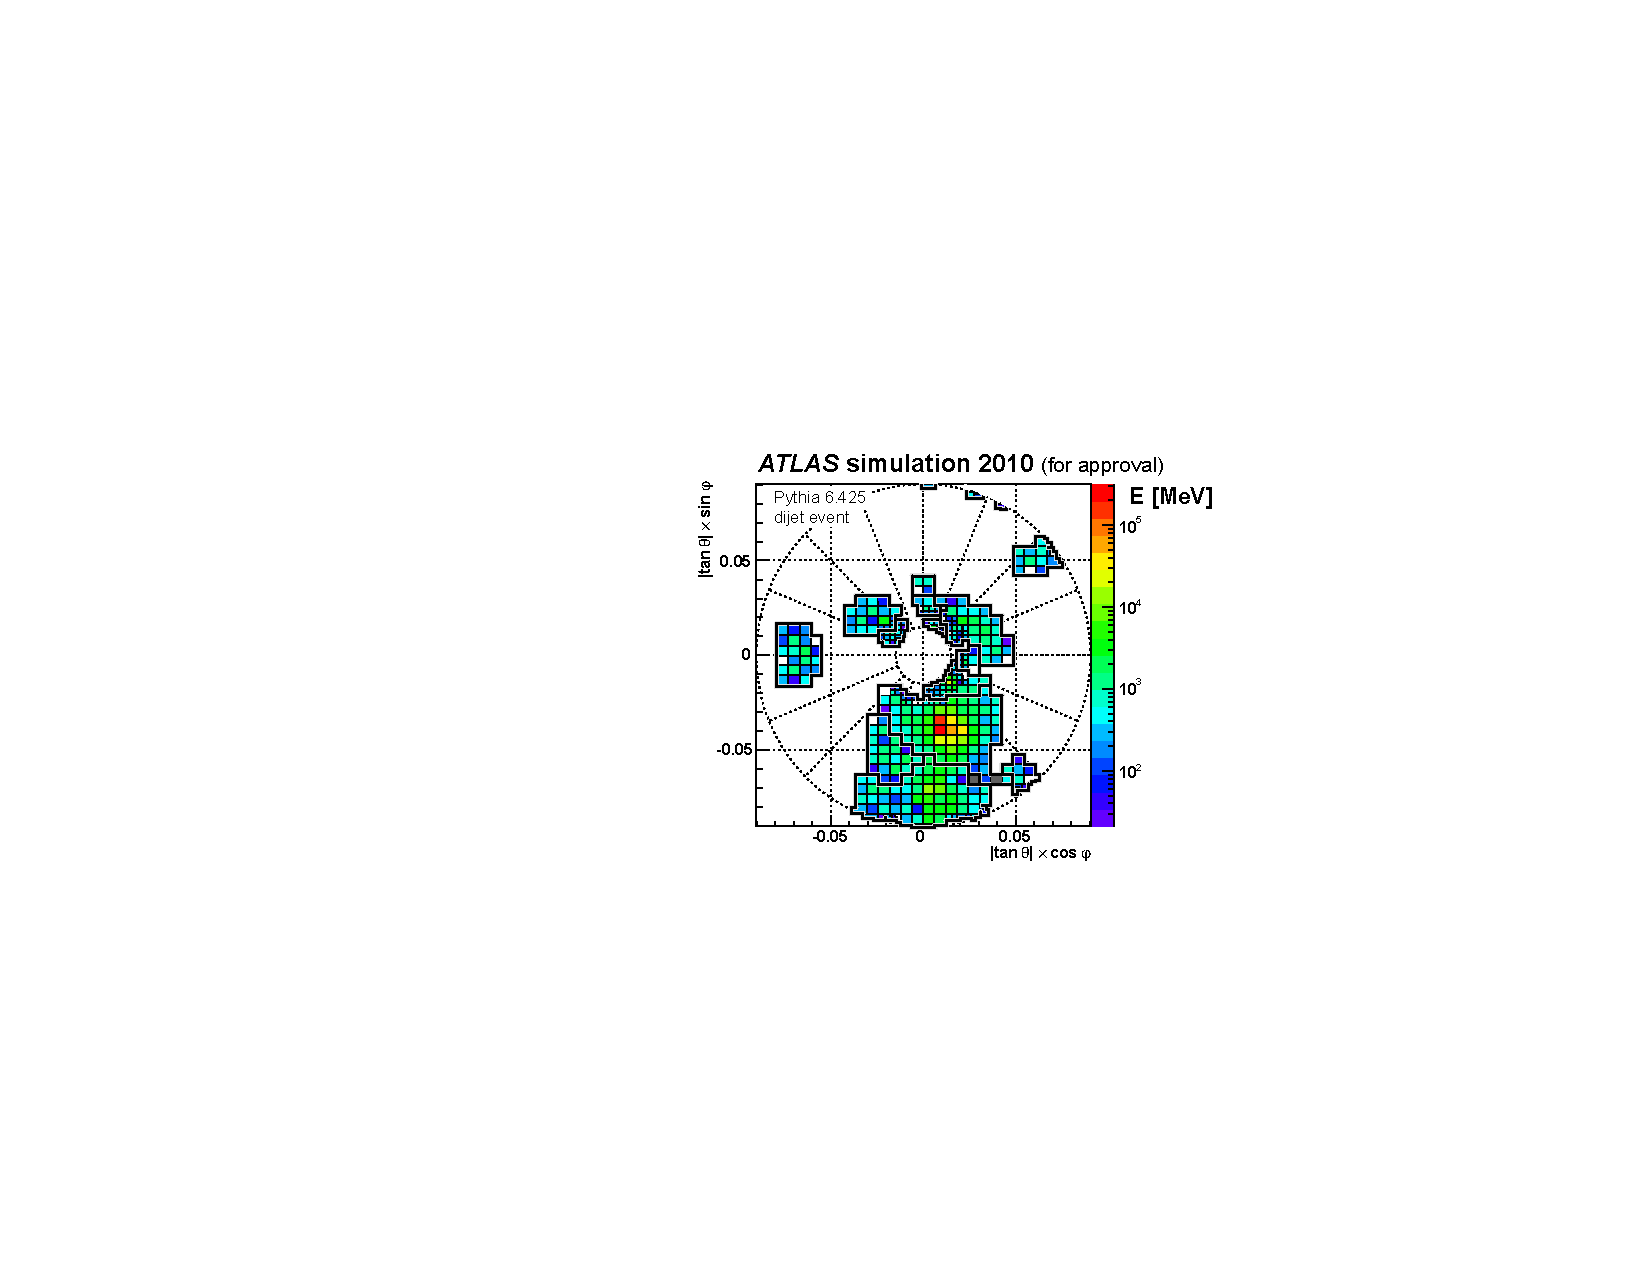
\includegraphics[width=0.6\textwidth]{FCal_evtdisplay_full.pdf}}
\label{fig:jet-reconstruction:jet-inputs:topoclustering-display}
\caption{Topo-cluster cells during the clustering, showing first the seed cells, then the growth cells, and finally all cells. Only the first layer of the LAR-FCal is shown in this event display. The final display also shows the outlines of the final topo-clusters, after splitting.}
\end{figure}

%%%%%%%%%%%%%%%%%%%%%

\subsection{Cluster Calibration}

Energy from electromagnetic particles (photons and electrons) is measured at a different scale from that of hadrons, whose interactions with material involve the release of nuclear binding and neutrinos which are not observed. Identifying clusters as originating from either of these two categories can improve the energy measurement, as type-dependent cluster calibrations can be applied to take into account these effects. This procedure is referred to as \textit{local calibration weighting}, as it uses local cluster information to calibrate the detector objects.

The identification of clusters as hadronic or EM uses a four-variable likelihood:
%
\begin{equation}
\mathcal{P}_\mathrm{clus}^\mathcal{EM}(E_\mathrm{clus}^\mathcal{EM}, \eta_\mathrm{clus}, \rho_\mathrm{clus},\lambda_\mathrm{center} ) \mapsto \mathcal{P}^\mathrm{EM}_{\mathrm{clus},ijkl} = \frac{N_{ijkl}^{\pi^0}}{N_{ijkl}^{\pi^0} + N_{ijkl}^{\pi^\pm}}
\end{equation}
%
where $E_\mathrm{clus}^\mathcal{EM}$ and $\eta_\mathrm{clus}$ are the cluster energy and position, and $\rho_\mathrm{clus}$ and $\lambda_\mathrm{center}$ are the cluster density and the radial depth of the cluster center. For a given energy and $\eta$, clusters with a lower radial depth and higher density are more likely to originate from EM particles, whereas hadronic interactions are expected to have longer and deeper showers. Neutral pions, which decay to photons, are used to train the EM particles in the likelihood, and positive pions are used to train the hadronic component. Figure~\ref{fig:jet-reconstruction:cluster-calibration:em-like} shows an example of the likelihood to be an EM shower, for a particular energy and $\eta$ bin. A cut on $\mathcal{P} > 0.5$ is typically used as the boundary of the classifier.

%%%%%%%%%%%%%%%%

\begin{figure}
\centering
\includegraphics[width=0.7\textwidth]{emlike.pdf}
\label{fig:jet-reconstruction:cluster-calibration:em-like}
\caption{An example of the likelihood used for classification of EM vs hadronic showers, for a particular bin of energy and $\eta$. The diagonal line indicates the surface of a $\mathcal{P} > 0.5$ cut.}
\end{figure}

%%%%%%%%%%%%%%%% 

After a cluster has been classified as hadronic or electromagnetic,  calibrations can be used to refine their energy measurement. There are three separate stages of calibration, as displayed in Figure~\ref{fig:jet-reconstruction:cluster-calibration:calib-flow}: hadronic calibration (if applicable), out-of-cone corrections, and dead material corrections.

%%%%%%%%%%%%%%%%

\begin{figure}
\centering
\includegraphics[width=0.7\textwidth]{calib_flow_cropped.pdf}
\label{fig:jet-reconstruction:cluster-calibration:calib-flow}
\caption{The form of the calibration algorithm for clusters in the LCW procedure.}
\end{figure}

%%%%%%%%%%%%%%%% 

The hadronic calibration weight, defined as $w_\mathrm{cell}^\mathrm{had} = \frac{{E}^\mathrm{dep}_\mathrm{cell}}{E^\mathrm{EM}_\mathrm{cell}}$, where the numerator is the truth amount of energy released in a shower, and the denominator is the measured amount. Look-up tables, created with single pion events, are developed for every cell in the detector in bins of the cell energy.

The out-of-cluster correction is used to account for energy which may be lost due to the significance cuts in the topo-clustering procedure. The correction is determined separately for EM and hadronic clusters, and single particle MC simulations are used to determine the size of the corrections. A specially designed search algorithm is used to find unassigned cells close to clusters which are likely part of the same shower, and adds their energy back to the cluster.

A final correction, again developed separately for EM and hadronic particles using single particle simulation, accounts for dead material in front of the calorimeters. The energy lost in these regions is found, in these simulations, to be strongly proportional to the energy in the pre-sampler, or the first layer of the FCal in the forward ergion. Additionally, energy lost in the transition regions between the EM and hadronic calorimeters is found to be proportional to $\sqrt{E_l^\mathrm{EM} E_f^\mathrm{had}}$, where $E_l^\mathrm{EM}$ is the energy in the last layer of the EM calorimeter, and $E_f^\mathrm{had}$ is the energy in the first layer of the hadronic calorimeter. Figure~\ref{fig:jet-reconstruction:cluster-calibration:ooc-dm} shows an example of the search strategies for both out-of-cluster and dead material corrections. 

%%%%%%%%%%%%%%%%

\begin{figure}
\centering
\includegraphics[width=0.7\textwidth]{ooc_dm_bounds.pdf}
\label{fig:jet-reconstruction:cluster-calibration:ooc-dm}
\caption{An example of the search procedures for the out-of-cluster and }
\end{figure}

%%%%%%%%%%%%%%%% 


Each cell in a cluster then has a continuous calibration weight, based on the cluster's $\mathcal{P}$, as:
%
\begin{equation}
w_\mathrm{cell}^\mathrm{cal} = \mathcal{P}^\mathrm{EM}_\mathrm{clus} w_\mathrm{cell}^\mathrm{em-cal} + (1 - \mathcal{P}_\mathrm{clus}^\mathrm{EM}) w_\mathrm{cell}^\mathrm{had-cal}
\end{equation}
%
where the individual $w_\mathrm{cell}$ terms are the products of the calibration factors previously described, for EM and hadronic showers. The final calibrated cluster then has the energy:
%
\begin{equation}
E^\mathrm{cal}_\mathrm{clus} = \sum_{i \in \mathrm{cluster}} w_{\mathrm{cell},i}^\mathrm{cal} E_{\mathrm{cell},i}^\mathrm{EM}
\end{equation}
%
which is just the sum of the individual cell energies with their respective weights. The cluster $\eta$ and $\phi$ are calculated using the cell weights in a similar way.

Most analyses which use substructure information use clusters calibrated to the LC scale: the calibration procedure brings particles much closer to their true energy, and removes at least some of the bias in which hadronic particles are measured at an incorrect scale. LC jets still require a JES calibration, described in the following sections, which indicates that the LC scale is not the complete truth scale: however, as substructure moments are calculated over all the constituents of a jet and usually normalized by the sum of their energies, it is most important that all particles be at a \textit{consistent} scale, which the LC calibration procedure largely accomplishes.

\subsection{Tracking}
\label{tracking}

Tracks are objects constructed from \textit{hits} in the inner detector: each hit corresponds to a particle interaction with a detector, and tracks correspond to the trajectories of these particles as they pass through. A number of sequential algorithms are used to find the tracks~\cite{Track2011,TrackOld}. The first is an ``inside-out'' algorithm which starts with 3-point seeds (colinear hits in either the pixel or SCT detectors, found with a fast seeding algorithm) and uses a Kalman filter to then iteratively add successive possible hits found along an extrapolated ``road'' in the detector. Each hit added to the track updates the track properties, and helps determine better the probable location of the next hit. Simultaneously, hits which dramatically increase the $\chi^2$ of the fit are rejected. Ambiguties can occur in the track matching, especially in the dense environments of jets; these are resolved before the track is extrapolated into the TRT. A second, ``outside-in'' algorithm starts with TRT seeds and extrapolates inwards; this algorithm produces significantly less well measured tracks.

Tracks used in analyses are required to pass a number of quality criteria, which unfortunately can vary from analysis to analysis. Typically, the quality requirements for jet measurements (non $b$-tagging) are:

\begin{enumerate}
\item $p_T > 500$~\MeV
\item $z_0 \sin{(\theta)}~<~$1.5 mm (relaxed for the purposes of JVF)
\item $d_0 < 1$~mm (relaxed for the purposes of JVF)
\item At least 1 pixel hit
\item At least 6 SCT hits
\item $\chi^2/$ndf $< 3$
\end{enumerate}

Tracks can be used in hadronic meaurements in many ways. Often, they are used as stand-alone inputs to jet algorithms, producing independent jets unbiased by the calorimeter measurements. Tracks can also be associated to jets, in order to measure additional properties of already determined calorimeter jets. Tracks are associated to jets typically in two ways: a $\Delta R$ association, or a ``ghost'' association. In the former, a distance between the track and jet axis is measured using the standard $\Delta R$ definition; tracks with $\Delta R < R_\mathrm{jet}$ are considered as associated to the jet. The ghost association technique is more complicated, and requires the concept of a \textit{jet area} to be defined, and so is described in Section~\ref{jet-reconstruction:pileup:ghost-association}.

% Previous studies of tracking performance in a low pile-up environment have demonstrated excellent algo- rithmic performance and good agreement between data and simulation [13, 14]. Tracks are reconstructed in the inner detector using a sequence of algorithms [15]. The inside-out algorithm starts from 3-point seeds in the silicon detectors and adds hits moving away from the interaction point using a combinato- rial Kalman filter. Ambiguities in the track candidates found in the silicon detectors are resolved, and tracks are extended into the TRT. The inside-out algorithm is the baseline algorithm designed for the efficient reconstruction of primary charged particles. Primary particles are defined as particles with a mean lifetime of greater than 3×10−11 s directly produced in a pp interaction or from the subsequent decays or interactions of particles with a lifetime shorter than 3 × 10−11 s. The tracks reconstructed by the inside-out algorithm are required to have transverse momentum pT > 400 MeV.
% In a second stage, a track search starts from segments reconstructed in the TRT and extends them inwards by adding silicon hits, which is referred to as back-tracking. Back-tracking is designed to re- construct secondaries, which are particles produced in the interactions of primaries. Finally tracks with a TRT segment but no extension into the silicon detectors are referred to as TRT-standalone tracks. This document focus on the impact of pile-up on the baseline inside-out algorithm. There is significant impact from pile-up on both back-tracking and TRT-standalone reconstruction, which will not be discussed here.


\section{Jet Calibration}

Once a jet has been clustered, from either EM-scale or LC-scale constituents, it is not yet ready for use by analyses. The non-compensating nature of the ATLAS calorimeters guarantees that the energy measured by the detectors is not the full energy of the particles which passed through them. Jets on ATLAS therefore go through several stages of additional corrections and calibrations, as outlined in Figure~\ref{fig:jet-reconstruction:making-jets}. Each level of the corrections and calibrations is referred to as a \textit{scale}. The steps involved are:

\begin{enumerate}
	\item Jet clustering, producing jets at the \textit{constituent scale} (or EM/LC)
	\item Jet areas pileup correction, and a residual NPV and $\mu$ dependent offset, producing jets at the \textit{pileup corrected scale}
	\item A jet origin correction, correcting the $\eta$ of a jet for the true location of the primary vertex, creating jets at the \textit{origin corrected scale}
	\item A Monte Carlo based \textit{Jet Energy Scale} (JES) calibration, producing jets at the \textit{particle scale}
	\item A Global Sequential Calibration to reduce flavor and hadronization sensitivity
	\item In-situ data-driven calibrations, producing jets at the \textit{fully calibrated scale}
\end{enumerate}

All of these steps are applied in ATLAS to $R=0.4$ and $R=0.6$ jets, using both EM and LC-scale inputs. While the LC calibration of the clusters is able to correct for non-compensation to some extent (by noting the difference between hadronic and electromagnetic interactions in the calorimeter, and the corresponding different energies they deposit), even LC-scale jets require significant further calibrations to correspond to truth jets. \LargeR jets, as used by the analyses in this thesis, undergo only the MC JES calibration, for reasons discussed below. The following sections describe each of these steps in detail.

%%%%%%%%%%%%%%%%

\begin{figure}
\centering
\includegraphics[width=0.9\textwidth]{JES_calib_chain.png}
\label{fig:jet-reconstruction:making-jets}
\caption{A diagram displaying the multiple steps which are used to transform a jet at the constituent scale to a fully-calibrated physics object for use in analysis.}
\end{figure}

%%%%%%%%%%%%%%%% 

\subsection{Pileup Corrections}

The first stage of jet calibration is to correct for pileup. As the calorimeter has a poor pointing resolution\footnote{Except with the notable exception of the ECal presampler, though this information is still limited and not yet used for pileup identification.}, it is not possible to determine which primary vertex (the hard-scatter, or pileup) an energy deposit originated from. This means that as a calorimeter jet is clustered, it contains energy from both the interaction of interest and the additional less-interesting interactions which occurred during the same bunch crossing. Even if a particle-flow algorithm is used to replace charged hadrons with their tracker measurements, thereby allowing a charged-hadron subtraction using the vertex identification of the tracks, neutral pileup particles cannot be subtracted and will add energy to the jet. \editnote{Cite this}

Jet pileup corrections are a broad topic of active research in both the theoretical and experimental community. \editnote{cite cite} The approach currently used by ATLAS is referred to as the \textit{jet areas} technique~\cite{jetareas}. The basic approach is to measure, event-by-event, the \textit{energy density} $\rho$ in the calorimeter. Though the underlying event contributes, at moderate and higher ($\mu > 10$, approximately) numbers of interactions, the contribution due to pileup to the energy density is dominant. Once the event energy density is measured, and the \textit{jet area} is measured, it is a simple matter to multiply the two and subtract off the pileup contribution to a jet.

The energy density can be measured in many ways. One approach, currently favored in the theory community, is simply to use sliding grid-shaped windows to scan the calorimeter, measuring the total energy deposit in each window, and then taking the median. The median is the best estimate of the ambient energy: measures such as the mean can be biased by the actual hard-scatter jets in the event. The approach used by ATLAS is similar, and follows an older prescription from the authors: the event is clustered into \kt $R=0.4$ jets, and each of their areas is calculated using the \textit{voronoi} technique (described below). The energy/area is calculated for each jet, and the median is used as the energy density (again in order to exclude outliers from real jets).

One detail of the topo-clustering algorithm creates an interesting effect when calculating the energy density. At approximately $\eta = 2.5$, the detector transitions from the barrel to the end-caps, which have a much higher expected noise due to pileup, as discussed in Section~\ref{jet-reconstruction:jet-inputs:topoclustering}. This, along with the reduced granularity in the forward regions, means that the energy density outside of jets decreases substantially: jets themselves are often still energetic enough to go over the noise thresholds required for topocluster formation, but pileup is often not. Thus, when calculating $\rho$, it is important to exclude the forward region of the detector, as the ambient energy outside of jets has greatly different characteristics than in the central region.

There are also several ways of calculating the area of jets, the simplest of which is the voronoi technique previously mentioned. A voronoi algorithm tiles a space (the calorimeter in $y-\phi$ space, in this case) such that each tile contains only one element (i.e., only one topocluster), and each tile contains all the points that are closest to that tile's element compared to any other~\cite{catchmentarea}. The voronoi area has the advantage of being fast to calculate, and gives (on average) the same value as more expensive calculations. The largest issue is that the algorithm does not take into account the energy of each element, which does not reflect the fact that the $k_T$ distance metrics generally do use energy.

A more sophisticated treatment of the area of a jet asks the question ``if a particle with very, very low energy were is at some position $y,\phi$, which jet (if any) would it join?'' This concept is at the heart of the \textit{catchment area} of a jet~\cite{catchmentarea}. To measure this area, special \textit{ghost particles} representing locations in the calorimeter participate in the jet clustering. The ghost particles have negligible energy (typically set to some $\epsilon$ value above 0), and so the IRC safety of the $k_T$ algorithms guarantee that the ghosts do not affect the clustering of the real jets. Once the mixture of ghost particles and real particles is clustered, one can examine which jet the ghost particle joined. When enough ghosts are used, this can be used to define the area of a jet (up to some level of coarseness). If the ghosts representing all the different calorimeter points are all simultaneously clustered with the real particles, this is referred to as the \textit{active area}; if on the other hand each point is added to the particles individually, and a separate clustering run each time, this is referred to as the \textit{passive area}. Both techniques are much slower than the Voronoi area calculation, and the passive calculation is again much slower than the active. The best compromise in terms of performance and usefulness of results seems to be the active area, and this is the definition used by ATLAS. The catchment area solves the issue observed with the Voronoi area: jet boundaries are determined by the algorithm's properties, and not just the closest point of a cluster. \Antikt jets, for example, form circles in $y-\phi$, and overlapping jets favor the higher $p_T$ jet: the $p_T$ weighting of the algorithm means that if a particle could join one of two jets, it will join the one with more energy. Figure~\ref{fig:jet-reconstruction:jet-active-areas} shows an event display with the areas of many \antikt $R=1.0$ jets and their \kt $R=0.3$ subjets: the circular nature of the \antikt algorith, and the more chaotic nature of \kt, are both visible.

%%%%%%%%%%%%%%%%

\begin{figure}
\centering
\includegraphics[width=0.6\textwidth]{jet-areas-example.pdf}
\label{fig:jet-reconstruction:jet-active-areas}
\caption{An event display showing a Pythia QCD simulation event with \antikt $R=1.0$ trimmed jets, with subjets formed by the \kt algorithm with $\Rsub = 0.3$.}
\end{figure}

%%%%%%%%%%%%%%%% 

Once the jet area and the energy density are known, the jet can be corrected. There are two approaches to this-- the simpler one is referred to as the scalar correction, and is applied with:
%
\begin{equation}
p_T^{\mathrm{corrected}} = p_T - \rho A
\end{equation}
%
where $A$ is the scalar area of the jet. It is also common to define the 4-vector $A_\mu$ by treating each ghost as a 4-vector and taking the sum of all of these; this allows for the 4-vector correction:
%
\begin{equation}
p_\mu^{\mathrm{corrected}} = p_\mu - \rho A_\mu
\end{equation}
%
Often this is preferable, as not just the $p_T$ but the mass of the jet is thus corrected for pileup. However, in some situations it is possible for the jet mass to be over-corrected, resulting in a negative $m^2$ and therefore imaginary mass. For this reason, ATLAS used only the scalar correction in Run~1. After the pileup correction, a jet is referred to as being at the ``pileup corrected scale'' and is ready for further calibration. Figure~\ref{fig:jet-reconstruction:jet-pu-vs-mu} shows the improvement in the RMS of the jet offset-- a measurement of the resolution induced by pileup-- as a function of $\mu$. The corrected distribution in blue shows a substantial improvement over the original distribution in black, and an average NPV based correction in red.

%%%%%%%%%%%%%%%%

\begin{figure}
\centering
\includegraphics[width=0.6\textwidth]{pu_vs_mu.pdf}
\label{fig:jet-reconstruction:jet-pu-vs-mu}
\caption{The improvement of the width of the jet offset (a measurement of the jet resolution in simulation) from the application of the jet areas pileup correction in blue, compared to an NPV based correction in red, and no correction in black.}
\end{figure}

%%%%%%%%%%%%%%%% 

One important aspect to note is that these corrections are done on jet 4-vectors as a whole, and not on constituents-- this means that jet moments, such as substructure observables, are not corrected. There are several extensions of the areas technique which aim to correct shapes, and some additional ideas which correct jet inputs before clustering, and therefore automatically correct shapes. While ATLAS explored some of these options in Run 1, the susceptibility of most variables to pileup was found to be rather small, putting off the need for dedicated corrections to Run 2. \editnote{Cite David's paper, others}

% plots plots? summarizing this?


\subsubsection{Aside: Ghost Association}
\label{jet-reconstruction:pileup:ghost-association}

Now that the concept of the jet area has been defined, it is possible to define the ghost association technique previously aluded to. This technique uses the active jet area, as defined with ghosts defined previously, to determine whether a track (or truth particle, etc.) should be associated to a jet. In particular, a track (or any other object) is replaced with a ghost copy-- i.e. one with the same physical position, but some small $\epsilon$ of energy. This ghost particle is allowed to participate in the jet clustering, and the jet which the ghost is clustered to identifies which jet the track should be associated with. Figure~\ref{fig:jet-reconstruction:ghost} is an event display showing such a matching of tracks to jets: even the complicated subjet shapes are able to have an unambiguous matching using the ghost association technique.


%%%%%%%%%%%%%%%%

\begin{figure}
\centering
\includegraphics[width=0.6\textwidth]{AKT10_legend4moment_example_etaphi_default.png}
\label{fig:jet-reconstruction:ghost}
\caption{An example of the ghost association algorithm in action, showing the locations of tracks from pileup vertices and from the hard-scatter vertices overlaid on the area of calorimeter jets. Tracks within the grey areas are considered to be associated to a jet.}
\end{figure}

%%%%%%%%%%%%%%%% 



Isolated \antikt jets are circular in shape, which motivates the $\Delta R$ association, which is fast to compute and is very accurate for these simple cases. The ghost association technique is often useful for environments where jets are non-circular-- i.e., when using the \kt or \ca algorithms, or when jets are very dense and overlapping and therefore non-circular.



\subsection{Jet Origin Correction}
\label{jet-reconstruction:origin}
Before any other corrections are performed, the $\eta$ of a jet is first adjusted, to take into account for the measured $z$ location of the primary vertex:
%
\begin{equation}
\eta^\mathrm{corrected} = \eta^\mathrm{detector} - \frac{z_{PV} \cosh \eta^\mathrm{detector} }{r}
\end{equation}
%
where $z_{PV}$ is the $z$ location of the primary vertex, and $r$ is the ``center-magnitude'' of the jet (i.e., a weighted sum of the jet clusters which averages over their energies to give the radial distance away from the center of the detector). Figure~\ref{fig:jet-reconstruction:origin_correction} shows the impact of the correction on the $\eta$ resolution of the jet, which is quite substantial.

%%%%%%%%%%%%%%%%

\begin{figure}
\centering
\includegraphics[width=0.6\textwidth]{origin_correction.pdf}
\label{fig:jet-reconstruction:origin_correction}
\caption{The improvement in the $\eta$ resolution after the application of the jet origin correction; no change in $\phi$ resolution is observed, as expected.}
\end{figure}

%%%%%%%%%%%%%%%% 

This correction is in fact a first order Taylor approximation to a more complete correction, of the form:
%
\begin{equation}
\eta^\mathrm{corrected} = \mathrm{asinh} \left(\sinh \eta^\mathrm{det} - \frac{z_{PV} \cosh \eta^\mathrm{detector}}{r}  \right).
\end{equation}
%
In principle, such a correction is best applied at the \textit{cluster} level, so that the jet clustering algorithms are run on origin-corrected inputs. This strategy will hopefully be adopted during Run 2, but in the meantime, the jet as a whole is corrected as part of the calibration process. The Color Flow analysis described in Chapter~\ref{chapter:color} actually performs this cluster-level correction for a number of reasons, which will be discussed later.


\subsection{MC Jet Energy Scale}
\label{jet-reconstruction:jet-calibration-mc-jet-energy-scale}

The MC Jet Energy Scale is the next step of the jet calibration chain. The sampling and non-compensating nature of the ATLAS calorimeters means that the measured energy is only some fraction of the energy of the actual particles passing through the detector. Futhermore, as the detector technology changes as a function of $\eta$, topoclusters in different parts of the detector may be better or worse measured, leading to biases in the jet direction. The JES is a correction which restores (on average) both this full energy, and correct direction, of a measured jet~\cite{JES2010}. The calibration is a multiplicative correction on energy, and an additive correction on $\eta$, binned in both the reconstructed jet energy and $\eta$.

Jets, composed of either EM or LC-scale clusters, are calibrated to the particle scale\footnote{From now on, reconstructed jets will refer to jets of both EM and LC consituents.} in Pythia 8 dijet events. This requires that the reconstructed jets are matched to truth jets. The requirement for matching is such that the $\Delta R$ between the reconstructed and truth jet is $<0.75\times R$. Furthermore, the matched jets (both truth and reconstructed) are also required to be isolated, such that no other jet of its type exists within $\Delta R < 2.5\times R$. All well matched jets within the sample are used. The dijet sample is used because it produces a well-understood spectrum of jets at many energy scales. The energy response is defined as:
%
\begin{equation}
\mathcal{R}^{\mathrm{jet}} = E^{\mathrm{jet}}_{\mathrm{reco}} /  E^{\mathrm{jet}}_{\mathrm{truth}} 
\end{equation}
%
and is measured in fine bins of $\eta_{\mathrm{detector}}$\footnote{The detector $\eta$ is used as it corresponds better to the location of the jet in the calorimeter.} and $E^{\mathrm{jet}}_{\mathrm{truth}}$. Each bin produces a Gaussian distribution, which is fit and the mean value is extracted. Each $E^{\mathrm{jet}}_{\mathrm{truth}}$ point in an $\eta$ bin then is then transformed into the corresponding $E^{\mathrm{jet}}_{\mathrm{reco}}$ point by this measured response-- this step is the ``numerical inversion'' which gives the technique its name. An entire $\eta$ bin is then fit by a log-polynomial function, of the form
%
\begin{equation}
\mathcal{F}_\mathrm{calib}\left(E^{\mathrm{jet}}_{\mathrm{reco}}\right) = \sum_{i=0}^N a_i \ln \left( E^{\mathrm{jet}}_{\mathrm{reco}} \right)^i
\end{equation}
%
where $N$, the maximum order of the polynomial, extends from 1 to 6 and is determined by minimizing the $\chi^2/$NDF of each fit. Finally, this function is inverted to get the calibration correction:
%
\begin{equation}
E^{\mathrm{jet}}_{\mathrm{JES}} = \frac{E^{\mathrm{jet}}_{\mathrm{reco}}}{\mathcal{F}_\mathrm{calib}}.
\end{equation}
%
Figure~\ref{fig:jet-reconstruction:e-fit} shows an example of the Gaussian fit used to find the response in each energy and $\eta$ bin; Figure~\ref{fig:jet-reconstruction:ni-e} shows the result of an example fit for the full energy distribution in the same $\eta$ bin. Figure~\ref{fig:jet-reconstruction:calib-function} shows the calibration function for all of the standard jet collections for one bin of $\eta$. Finally, Figure~\ref{fig:jet-reconstruction:total_jes} shows the JES for different energy bins as a function of the detector $\eta$, for both the EM and LC $R=0.4$ collections.

This is a rather complicated procedure, and a relevant question to ask is why the correction cannot be derived by simply measuring the correction factor directly in bins of $E$ and $\eta$, and skipping the numerical inversion steps. The numerical inversion technique, while introducing complexity, is preferred because it removes the dependence of the calibration on the input $p_T$ spectrum. If the correction were binned in $E_{\mathrm{reco}}$, then the truth-jets matched to the reconstructed jet will have both up-fluctuations and down fluctuations due to the calorimeter response, but there are more likely to be down fluctuations, because there are more low $p_T$ jets in the dijet sample than high $p_T$ jets. This introduces a bias due to the $p_T$ shape-- if that shape changes, as it does in a different physics sample, then the calibration would no longer be valid. On the other hand, if we bin in $E_{\mathrm{truth}}$ to start, then the fluctuations up and down will depend only on the calorimeter response-- the physics spectrum has already been accounted for by the $E_{\mathrm{truth}}$ binning.


%%%%%%%%%%%%%%%%

\begin{figure}
\centering
\includegraphics[width=0.6\textwidth]{e_fit.pdf}
\label{fig:jet-reconstruction:e-fit}
\caption{An example of the Gaussian fit used to measure the energy response in a $\eta_\mathrm{detector}$, $E_\mathrm{true}$ bin.}
\end{figure}

%%%%%%%%%%%%%%%% 


%%%%%%%%%%%%%%%%

\begin{figure}
\centering
\includegraphics[width=0.6\textwidth]{ni_e.pdf}
\label{fig:jet-reconstruction:ni-e}
\caption{An example of the log-polynomial fit used to measure the jet response as a function of $E_\mathrm{reco}$ in a bin of $E_\mathrm{detector}$. The inverse of this function is the energy calibration applied for each point.}
\end{figure}

%%%%%%%%%%%%%%%% 

%%%%%%%%%%%%%%%%

\begin{figure}
\centering
\includegraphics[width=0.6\textwidth]{calib_function.pdf}
\label{fig:jet-reconstruction:calib-function}
\caption{The size of the calibration constants for each of the standard jet collection for one bin of $\eta_\mathrm{detector}$.}
\end{figure}

%%%%%%%%%%%%%%%% 

%%%%%%%%%%%%%%%%

\begin{figure}
\centering
\subfigure[EM]{\includegraphics[width=0.45\textwidth]{figures/jet-reconstruction/total_jes_eta_em.pdf}}
\subfigure[LC]{\includegraphics[width=0.45\textwidth]{figures/jet-reconstruction/total_jes_eta_lc.pdf}}
\label{fig:jet-reconstruction:total_jes}
\caption{The size of the calibration constants for each of the standard jet collection for one bin of $\eta_\mathrm{detector}$.}
\end{figure}

%%%%%%%%%%%%%%%% 

The $\eta$ correction mentioned previously is derived as a subsequent correction in much the same way, except that the response is defined additively:
%
\begin{equation}
\mathcal{R}_\eta^\mathrm{jet} = \eta^{\mathrm{jet}}_{\mathrm{reco}} -  \eta^{\mathrm{jet}}_{\mathrm{truth}} 
\end{equation}
%
and the correction is therefore also additive. The size of the correction is not large in the central region, where the uniform detector technology leads to consistently measured clusters, but becomes important especially in the tranisition regions between detectors. Figure~\ref{fig:jet-reconstruction:eta-fit} shows an example of the Gaussian fit used to determine the response; Figure~\ref{fig:jet-reconstruction:ni-eta} shows an example of the calibration function itself in an $\eta$ bin where the correction is non-negligible. Finally, Figure~\ref{fig:jet-reconstruction:total-eta} shows the full size of the correction for different energy bins as a function of $\eta$ for $R=0.6$ EM jets in 2010-- the correction is similar in 2012 conditions.

%%%%%%%%%%%%%%%%

\begin{figure}
\centering
\includegraphics[width=0.6\textwidth]{eta_fit.pdf}
\label{fig:jet-reconstruction:eta-fit}
\caption{An example of the Gaussian fit used to measure the $\eta$ response in a $\eta_\mathrm{detector}$, $E_\mathrm{true}$ bin.}
\end{figure}

%%%%%%%%%%%%%%%%

%%%%%%%%%%%%%%%%

\begin{figure}
\centering
\includegraphics[width=0.6\textwidth]{ni_eta.pdf}
\label{fig:jet-reconstruction:ni-eta}
\caption{An example of the log-polynomial fit used to measure the jet $\eta$-response as a function of $E_\mathrm{true}$ in a bin of $E_\mathrm{detector}$. The jet-$\eta$ correction is the negative of each point.}
\end{figure}

%%%%%%%%%%%%%%%% 

%%%%%%%%%%%%%%%%

\begin{figure}
\centering
\includegraphics[width=0.6\textwidth]{total_eta.pdf}
\label{fig:jet-reconstruction:total-eta}
\caption{The full size of the $\eta$ calibration corrections, for different bins of energy and as a function of the detector $\eta$, for $R=0.6$ EM jets in 2010.}
\end{figure}

%%%%%%%%%%%%%%%% 

% If you bin in reco, you match truth to your reco jet. because your smaple has a a pt spectrum, you will match more low truth than high truth (though calorimter response means that you will have both up and down). this is a bias. if you bin in truth, the fluctuation up and down will be equal-- the calorimeter response will be the only thing causing up/down. thus, if your correction is binned in truth, it will not be biased, but it requires a numerical inversion to do correctly.


\subsection{Global Sequential Calibration}
\label{jet-reconstruction:calibration:gsc}

Jets are calibrated to the particle scale in an inclusive dijet sample, which has a particular quark/gluon composition. Due to their different showering and hadronization properties-- gluons first split to quarks, and therefore typically have higher (but softer) particle multiplicities-- quark and gluon jets will have a different response in the detector\footnote{See Section~\ref{jet-reconstruction:qg} for a much large discussion of quark/gluon jet differences, and a more precise treatment of the exact labeling used to define these.} The Global Sequential Calibration of jets, following the JES, is a correction which uses measurable properties of jets to reduce this sensitivity to different types of hadronization, and therefore to quark/gluon flavor induced miscalibration~\cite{ATLAS-GSC}. Moreover, even jets of a single flavor type can fragment in wildly different ways, resulting in a range of possible responses: by measuring global jet properties, it is possible to better understand this fragmentation and correct the response jet-by-jet and thereby substantially improve the jet resolution.

Five variables are used to correct the jets; most of the variables are only available in some subset of the detector $\eta$. As the name of the technique suggests, these corrections are applied independently and sequentially. In order, these are:

\begin{enumerate}
	\item In $0 < |\eta| < 1.7$, $f_{\mathrm{Tile0}}$, the fraction of energy in the first layer of the tile calorimeter.
	\item In $0 < |\eta| < 3.5$, $f_{\mathrm{LAr3}}$, the fraction of energy in the third layer of the LAr EM calorimeter.
	\item In $0 < |\eta| < 2.5$, \ntrk, the number of primary-vertex tracks associated to a jet.
	\item In $0 < |\eta| < 2.5$, Track Width, the radial distribution of the $p_T$ of tracks associated to a jet, defined as:
	\begin{equation}
	\mathrm{Track~Width} = \frac{\sum_{i \in j} p_T^{i} \Delta R(i,j) }{\sum_{i \in j} p_T^i}
	\end{equation}
	where $i$ iterates over tracks associated to jet $j$.
	\item In $0 < |\eta| < 2.7$, $N_\mathrm{segments}$, the number of muon segments associated to a jet
\end{enumerate}
The first two variables, $f_{\mathrm{Tile0}}$ and $f_{\mathrm{LAr3}}$, measure the longitudinal shower profile of the jet. \ntrk measures the charged component of the jet fragmentation; the track width measures the shower profile in the $\eta-\phi$ plane. $N_{\mathrm{segments}}$ measures the amount of hadronic activity in the muon spectrometer, a result of so-called ``punch-through'' wherein not all hadrons are stopped and sampled by the calorimeters. Because LC jets already contain longitudinal information in the topo-clusters, the first two variables are ommitted for the GSC for that class of jets. Figure~\ref{fig:jet-reconstruction:gsc} shows the dependence of the jet response on these variables. The correction, as a function of the variable $x$, is defined as $C(x) = \mathcal{R}^{-1}(x)$, where $\mathcal{R}$ is the \pt response. This correction is binned finely in both \pt and $\eta$, and is normalized such that the inclusive response does not change. After the calibrations, the average response is 1 when measured by any of these variables, indicating that the jet energy measurement variance has been substantially reduced. Figure~\ref{fig:jet-reconstruction:resolution_gsc} shows the improvement in the \textit{jet resolution} (i.e., the width of a response measurement) as a function of \pt; the lower values after the GS correction, in blue, compared to the nominal in black, indicate that fluctuations in jet measurement have been reduced.


\begin{figure}
\centering
\subfigure[$f_{\mathrm{Tile0}}$]{\includegraphics[width=0.3\textwidth]{fig_06a.pdf}}
\subfigure[$f_{\mathrm{LAr3}}$]{\includegraphics[width=0.3\textwidth]{fig_06b.pdf}}
\subfigure[\ntrk]{\includegraphics[width=0.3\textwidth]{fig_06c.pdf}}

\subfigure[Track Width]{\includegraphics[width=0.3\textwidth]{fig_06d.pdf}}
\subfigure[$N_\mathrm{Segments}$]{\includegraphics[width=0.3\textwidth]{fig_06e.pdf}}
\label{fig:jet-reconstruction:gsc}
\caption{The average jet response, as a function of each GSC variable, in a central bin of jet $\eta$.}
\end{figure}

\begin{figure}
\centering
\includegraphics[width=0.6\textwidth]{fig_04a.pdf}
\label{fig:jet-reconstruction:resolution_gsc}
\caption{The improvement in jet resolution after applying the GSC correction.}
\end{figure}


\subsection{In-situ Calibrations and Uncertainty Derivation}
\label{chapter:jet-reconstruction:insitu}

Following the JES and GSC calibration steps, a final data-driven \textit{in-situ} calibration uses different jet balance techniques in data to develop a small residual correction and a measurement of the uncertainties on the final jet $p_T$ scale. $Z$+jet, $\gamma$+jet, and multi-jet measurements are used in low $p_T$, medium $p_T$, and high $p_T$ regions respectively.

In $Z$+jet measurements, a well reconstructed $Z$-boson, decaying in either the $e^+/e^-$ or $\mu^+/\mu^-$ channel, is used as a reference object to probe the quality of the jet energy measurement. In particular, a reference \pt is defined as $p_T^\mathrm{ref} = p_T^\mathrm{Z} \times |\cos(\mathrm{jet}, Z) |$ in order to take into account the potential presence of additional parton radiation which might affect the direct balance of the $Z$ and the leading jet. The mean of the response (defined as $\mathcal{R}_Z = p_T^\mathrm{jet} / p_T^\mathrm{ref}$) is measured using Poisson fits at low $p_T^\mathrm{ref}$ (due to inefficiency of the trigger cutting off the low end of the response) and the arithmetic mean at higher values; the disagreement between data and MC, as a function of $p_T^\mathrm{ref}$, is used to estimate the systematic uncertainty on the jet $p_T$. Figure~\ref{fig:jet-reconstruction:z_jet} shows an example of one such fit in a bin of $p_T^\mathrm{ref}$, and of the evolution of $\mathcal{R}_Z$ as a function of $p_T^\mathrm{ref}$.

%%%%%%%%%%%%%%%%

\begin{figure}
\centering
\subfigure[Example of a fit used to estimate $\mathcal{R}_Z$]{\includegraphics[width=0.45\textwidth]{fig_15a.pdf}}
\subfigure[Data/MC as a function of $p_T^\mathrm{ref}$]{\includegraphics[width=0.45\textwidth]{fig_17a.pdf}}
\label{fig:jet-reconstruction:z_jet}
\caption{Examples of the measurements used to measure the uncertainties in jet $p_T$ at low \pt using $Z$+jet events.}
\end{figure}

%%%%%%%%%%%%%%%% 

The $\gamma$+jet measurements use a similar principle, and measures $\mathcal{R}_\gamma = p_T^\mathrm{jet} / p_T^\gamma$. High quality photon events are selected in both data and MC, and the $\mathcal{R}_\gamma$ is measured in both in fine bins of \pt and $\eta$. Poisson fits are used at low \pt because of trigger turn-on issues, and the arithmetic mean is used at higher values, to estimate the average response as a function of $p_T^\gamma$.  Figure~\ref{fig:jet-reconstruction:gamma_jet} shows an example of a fit to $\mathcal{R}_\gamma$ in one bin of $p_T^\gamma$ and the evolution of the mean value as a function of $p_T^\gamma$.

%%%%%%%%%%%%%%%%

\begin{figure}
\centering
\subfigure[Example of a fit used to estimate $\mathcal{R}_\gamma$]{\includegraphics[width=0.45\textwidth]{fig_22b.pdf}}
\subfigure[Data/MC as a function of $p_T^\gamma$]{\includegraphics[width=0.45\textwidth]{fig_23a.pdf}}
\label{fig:jet-reconstruction:gamma_jet}
\caption{Examples of the measurements used to measure the uncertainties in jet $p_T$ at moderate \pt using $\gamma$+jet events.}
\end{figure}

%%%%%%%%%%%%%%%% 

At high \pt, a multijet balance technique is used to derive uncertainties. In this technique, a leading jet with \pt significantly higher than a system of low \pt jets is balanced against that system; the uncertainties on the well-measured low \pt jets are propagated in order to estimate the \pt of the leading jet. The multijet balance is defined as $\mathrm{MJB} = \frac{|\vec{p}_T^{\mathrm{jet}}|}{|\vec{p}_T^{\mathrm{recoil}}|} $; events used in the analysis are required to have $p_T^\mathrm{leading}$ smaller than some fraction of $p_T^\mathrm{leading}$. The analysis procedeeds iteratively, starting with low $p_T^\mathrm{subleading}$ and proceeding higher as the uncertainties are successively iterated to higher values of $p_T^\mathrm{jet}$. Figure~\ref{fig:jet-reconstruction:mjb} shows the value of the MJB as a function of $p_T^\mathrm{jet}$ before any iterations; the residual disagreement between data and MC in this plot, after all iterations, is used as the uncertainty at high \pt.

%%%%%%%%%%%%%%%%

\begin{figure}
\centering
\includegraphics[width=0.6\textwidth]{fig_29a.pdf}
\label{fig:jet-reconstruction:mjb}
\caption{The value of the MJB, as a function of $p_T^\mathrm{recoil}$, in data and MC. The residual disagreement is used to define the uncertainty at high $p_T^\mathrm{jet}$.}
\end{figure}

%%%%%%%%%%%%%%%% 


Each of the previously mentioned techniques, as well as creating an uncertainty band on \pt, also can determine the mismeasurement of the scale, which is typically $0-2\%$. These corrections are applied to data only, bringing the data and MC to the same scale after the full calibration procedure.

Once each of these procedures is performed, they are statistically combined to create a total calibration and uncertainty. Each procedure is weighted, as a function of \pt and $\eta$, by the systematic and statistical uncertainty of that procedure: the combined calibration and uncertainty uses a measurement most heavily when its uncertainties are lowest. Figure~\ref{fig:jet-reconstruction:combined_jes} shows the result of this combination, and the applicable range of each measurement. This figure also shows the combined size of the residual calibration applied to data: a factor $C = 1/\mathcal{R}_\mathrm{in-situ}$, where $\mathcal{R}_\mathrm{in-situ}$ is the value on the y-axis of the figure, is applied to data in order to bring the response in data and MC to the same level.

%%%%%%%%%%%%%%%%

\begin{figure}
\centering
\includegraphics[width=0.6\textwidth]{responseRatio_LCJES_R4-2.pdf}
\label{fig:jet-reconstruction:combined_jes}
\caption{The combined uncertainty band, overlaid with the uncertainties derived from the $Z$+jets, $\gamma$+jets, and multijet analyses.}
\end{figure}

%%%%%%%%%%%%%%%% 

Figure~\ref{fig:jet-reconstruction:combined_uncertainties} shows the size of the uncertainties as a function of \pt and $\eta$: jets are measured best at central $\eta$ and at moderate \pt. The plots also show a breakdown of the physics sources of the uncertainties: pileup dominates at low \pt, but at higher values the in-situ measurements are largest (the relative \textit{in-situ} refers to the $\eta$-intercalibration used to provide uncertainties at high $\eta$, using an iterative technique similar to the MJB). Additional terms are usually provided for the variation due to the unknown flavor response and flavor composition; the use of the GSC calibrations help reduce those terms.

%%%%%%%%%%%%%%%%

\begin{figure}
\centering
\subfigure[As a function of $p_T^\mathrm{jet}$]{\includegraphics[width=0.45\textwidth]{JESUncertainty-Moriond2013-Dijet-LC4-pT-noCloseby.pdf}}
\subfigure[As a function of $\eta$]{\includegraphics[width=0.45\textwidth]{JESUncertainty-Moriond2013-Dijet-LC4-eta-noCloseby.pdf}}
\label{fig:jet-reconstruction:combined_uncertainties}
\caption{The combined JES uncertainty, as a function of \pt and $\eta$, in 2012 data, for \antikt~$R=0.4$ LC jets.}
\end{figure}

%%%%%%%%%%%%%%%% 


\subsection{\LargeR Calibrations}

The standard jet calibration chain is run only on $R=0.4$ and $R=0.6$ jets, using both LC and EM scale inputs. For analyses which require the use of jets with a different $R$ parameter and/or grooming, another set of calibrations must be performed. Optimization studies on a variety of signal classes in 2011 determined that the collection \antikt $R=1.0$ with trimming applied, using $\Rsub = 0.3$ and $\fcut = 0.05$, performed very well in a number of final states, and presented a very small susceptibility to pileup as demonstrated in Figure~\ref{fig:jet-reconstruction:pileup_large}~\cite{ATLAS-SS-2011}. This collection was thus centrally supported in 2012, and both calibrations and uncertainties were provided.

\begin{figure}
\centering
\includegraphics[width=0.6\textwidth]{fig_18b.pdf}
\label{fig:jet-reconstruction:pileup_large}
\caption{The dependence of the average lead jet mass in dijet events in 2011 data for ungroomed \antikt $R=1.0$ jets and several configurations of trimming.}
\end{figure}


The calibration procedure for these \largeR jets is slightly different than for the other collections. As most users are interested in the substructure properties of the jets, and using constituents at the hadron-scale is more sensible than the raw detector outputs, only LC inputs are used for \largeR jets. Additionally, because trimming effectively removes a large portion of the pileup contamination in the jets, no dedicated pileup correction procedure is applied (though in principle, it is possible to easily add an areas correction to the subjets before they are trimmed, and this should improve performance). This is visible in Figure, which shows the lack of sensitivity of the jet mass to additional pileup interactions. Thus, the MC JES procedure is performed on jets at the LC scale.

The MC JES procedure itself is identical to that described in Section~\ref{jet-reconstruction:jet-calibration-mc-jet-energy-scale}, except that an additional \textit{mass calibration} step is performed. This procedure defines a mass response in the typical way,
%
\begin{equation}
\mathcal{R}^{\mathrm{jet}}_m = m^{\mathrm{jet}}_{\mathrm{reco}} /  m^{\mathrm{jet}}_{\mathrm{truth}} 
\end{equation}
%
and performs a numerical inversion calibration procedure identical to the energy calibration procedure, after both the energy and $\eta$ are calibrated. This procedure is required because of the varying mass response of the calorimeter, as displayed in Figure~. This is again caused by the varying performance of detector technologies which change as a function of $\eta$: hadrons on one side of the jet, without a calibration, would cause more mass in the jet than the other side, even if they had the same energy. As the mass of \largeR jets is commonly used as a discriminating variable in analyses (as opposed to the $R=0.4$, which is rarely if ever used), it is important that the variable have a consistent meaning as the detector technology changes. Figure~\ref{fig:jet-reconstruction:total_jms} shows the effect of the jet calibration in 2011; while the mass response is close to $1$ in central $\eta$ bins, it can be substantially mismeasured at higher values of $\eta$ when the jet energy is low.

\begin{figure}
\centering
\subfigure[Before mass calibration]{\includegraphics[width=0.45\textwidth]{fig_07a.pdf}}
\subfigure[After mass calibration]{\includegraphics[width=0.45\textwidth]{fig_07b.pdf}}
\label{fig:jet-reconstruction:total_jms}
\caption{The mass response, for different bins of jet energy, as a function of jet $\eta$, before and after the calibration procedure.}
\end{figure}

Uncertainties on the \largeR jets are derived using a track-jet double ratio technique. Track-jets reconstructed with the same jet algorithm are matched to the calorimeter jets in a multi-jet sample, in both data and simulation. The ratio of the track-jet mass to the calorimeter mass is then measured: this provides a comparison of two indepenent measurements of the jet mass. The ratio of this ratio gives a bound on the disagreement of the modelling of the jet mass (or $p_T$, or other quantities) in the simulation.  These uncertainties, while conservative because of the introduction of charged fragmentation modeling, provide an \textit{in-situ} alternative measurement of the jet mass and other substructure properties. Figure~\ref{fig:jet-reconstruction:jms_uncertainty} shows both the raw track-to-calo mass ratio, and the corresponding derived uncertainty as a function of the jet \pt, in 2011 data.

%%%%%%%%%%%%%%%%%%%%%

\begin{figure}
\centering
\subfigure[Track/Calo Mass]{\includegraphics[width=0.45\textwidth]{fig_09b.pdf}}
\subfigure[Mass uncertainty]{\includegraphics[width=0.45\textwidth]{fig_10b.pdf}}
\label{fig:jet-reconstruction:jms_uncertainty}
\caption{The jet track mass/ calo mass ratio in data and MC as a function of the jet mass, and the corresponding derived uncertainty as a function of jet \pt.}
\end{figure}

%%%%%%%%%%%%%%%%%%%%%

\section{Pileup Jet Tagging}
\label{jet-reconstruction:pileup-jet-tagging}

While the jet areas pileup suppression is able to remove the ambient pileup energy within \textit{existing} jets, oftentimes pileup interactions can produce entirely new jets. There are two ways that this can happen. First, a pileup interaction can simply produce a dijet event with appreciable \pt: in this case, the jets are in some sense real, but come from an interaction different from the one of interest\footnote{Usually the primary interaction is defined as the vertex with the highest $\pt^2$ of its associated tracks.}. In other situations, particles produced by pileup interactions can by chance be concentrated in one location; in such a case, a new \textit{stochastic} jet is produced by the products of many interactions. In both situations, tracking information can be used (at least within the tracker acceptance) to measure the degree of pileup particles contributing to a jet.

The simplest method of meausuring this pileup contamination is with a variable called JVF, which is defined as:
%
\begin{equation}
\label{eqn:jet-reconstruction:jvf}
\mathrm{JVF} = \frac{\sum_k p_T^{\mathrm{trk},k}(\mathrm{PV}_0)}{ \sum_l p_T^{\mathrm{trk},l}(\mathrm{PV}_0) + \sum_{n\geq1} \sum_l p_T^{\mathrm{trk},l}(\mathrm{PV}_n)}
\end{equation}
%
where the sums over tracks ($k$ and $l$ indices) are tracks which are ghost-associated to a jet~\cite{ATLAS-JVF}. Thus, the variable is defined as the primary vertex track \pt fraction: the amount of \pt in a jet originating from the primary vertex, compared to all other vertices. An example distribution in 2012 conditions is shown in Figure~\ref{fig:jet-reconstruction:jvf}: real jets have a high fraction, as expected, and pileup jets have a low fractions. Jets without any tracks are assigned a value of $-1$. Analyses typically select jets with $|\mathrm{JVF}| > 0.5$, and apply this cut only when jets have $\pt < 50$ GeV, as the rate of high \pt pileup jets is exceedingly small. 

%%%%%%%%%%%%%%%%

\begin{figure}
\centering
\includegraphics[width=0.6\textwidth]{fig_26.pdf}
\label{fig:jet-reconstruction:jvf}
\caption{An example distribution of JVF measured for primary vertex and pileup jets in a $Z$+jets simulation sample.}
\end{figure}

%%%%%%%%%%%%%%%% 

One issue with JVF is that while it is indeed able to identify pileup jets, the second term in the denominator Equation~\ref{eqn:jet-reconstruction:jvf} depends on $N$, the number of pileup vertices in the event~\cite{ATLAS-JVT}. Ideally, pileup supression would be done using variables which are themselves not dependent on pileup, so that the efficiency and fake-rate of such variables do not change with the pileup conditions. One simple way to do this is to correct the problematic term in  Equation~\ref{eqn:jet-reconstruction:jvf}, defining a new variable corrJVF as:
%
\begin{equation}
\label{eqn:jet-reconstruction:corrjvf}
\mathrm{corrJVF} = \frac{\sum_k p_T^{\mathrm{trk},k}(\mathrm{PV}_0)}{ \sum_l p_T^{\mathrm{trk},l}(\mathrm{PV}_0) + \frac{\sum_{n\geq1} \sum_l p_T^{\mathrm{trk},l}(\mathrm{PV}_n)}{\kappa n_\mathrm{trk}^\mathrm{PU}}}
\end{equation}
%
where $\kappa$ is an arbitrary factor, typically selected to be 0.01, and $n_\mathrm{trk}^\mathrm{PU}$ is the \textit{total} number of pileup tracks in the event~\cite{ATLAS-JVT}. This normalization prevents the arbitrary growth of the second term, and renders corrJVF insensitive to the number of pileup tracks, and just as performant as JVF. Another variable which is sensitive to pileup jets, but insensitive to the number of vertices, is $R_{p\mathrm{T}}$, defined as
%
\begin{equation}
R_{p\mathrm{T}} = \frac{\sum_k p_T^{\mathrm{trk},k}(\mathrm{PV}_0)}{p_T^\mathrm{jet}}.
\end{equation}
%
This variable is the simply the charged component of the jet \pt~\cite{ATLAS-JVT}. For typical jets, 2/3 of the energy is expected to occur in charged particles (due to there being two charges, and only one neutral ``charge''), with some degree of flucutation due to charged hadronization and detector inefficiencies. A lower value indicates either a strangely fragmenting jets, or more dangerously, a large degree of pileup contamination. As corrJVF and $R_{p\mathrm{T}}$ contain orthogonal information-- one measures the pileup track contamination, and the other the neutral contamination-- the variables ccan be combined using a likelihood into a new, more powerful variable: JVT (the jet-vertex-tagger). The distributions of corrJVF, $R_{p\mathrm{T}}$, and JVT are showin in Figure~\ref{fig:jet-reconstruction:jvt}.

%%%%%%%%%%%%%%%%%%%%%

\begin{figure}
\centering
\subfigure[corrJVF]{\includegraphics[width=0.3\textwidth]{fig_02a.pdf}}
\subfigure[$R_{p\mathrm{T}}$]{\includegraphics[width=0.3\textwidth]{fig_03a.pdf}}
\subfigure[JVT]{\includegraphics[width=0.3\textwidth]{fig_05b.pdf}}
\label{fig:jet-reconstruction:jvt}
\caption{The distributions of various $N_\mathrm{vtx}$-insensitive pileup tagging variables.}
\end{figure}

%%%%%%%%%%%%%%%%%%%%%

The improvement in performance of JVT is shown in Figure~\ref{fig:jet-reconstruction:jvt_performance}~\cite{ATLAS-JVT}. The left figure shows the fake rate (i.e. the rate of acceptance of pileup jets) as a function of the hard-scatter jet efficiency-- a lower curve indicates stronger performance, and JVT clearly performs the best out of the different variables. The right figure shows the fake rate as a function of $N_\mathrm{vtx}$ for a fixed efficiency; the strong sensitivity of JVF is visible, while JVT is not affected.  

%%%%%%%%%%%%%%%%%%%%%

\begin{figure}
\centering
\subfigure{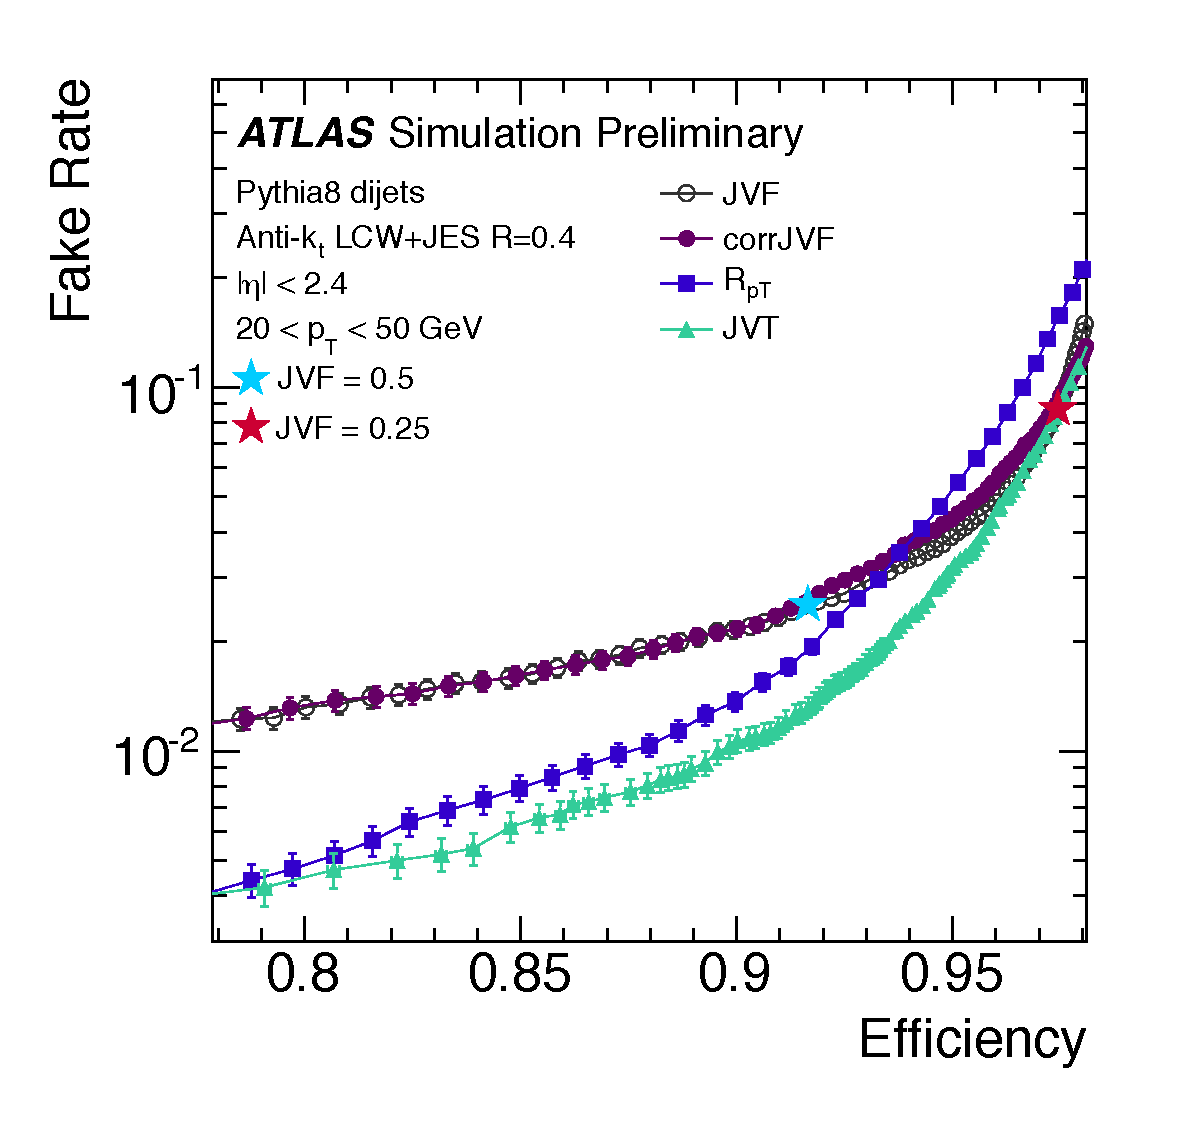
\includegraphics[width=0.45\textwidth]{fig_06a_jvt}}
\subfigure{\includegraphics[width=0.45\textwidth]{fig_06b_jvt}}
\label{fig:jet-reconstruction:jvt_performance}
\caption{Performance of JVT compared to JVF, comparing both the efficiency vs. fake-rate and the sensitivity to changing $N_\mathrm{vtx}$ conditions.}
\end{figure}

%%%%%%%%%%%%%%%%%%%%%

\subsection{Pileup in \LargeR Jets}

Typically \largeR jets are not directly sensitive to the creation of new pileup jets: the high \pt thresholds used in these analyses typically mean that jets consisting of entirely pileup are very rare. One possible issue is the presence of pileup \textit{subjets}: i.e., small subjets within an otherwise normal \largeR jet which are dominated by pileup~\cite{ATLAS-JVT}. Figure~\ref{fig:jet-reconstruction:pu_subjet} shows an example of such a jet: the \largeR jet labeled as the truth $Z$-boson (in this simulated $W'\rightarrow WZ$ event) has a mass of 90 GeV when using only the two subjets on the left, but rises to 120 when including the subjet on the right. However, it is also clear from this event display that the subjet on the right has no hard-scatter tracks associated to it, and only tracks from pileup interactions\footnote{This figure nicely demonstrates the advantage of the ghost-association scheme for tracks: the non-trivial shape of the \kt subjets are captured by the ghost association, but not by a simpler $\Delta R$ scheme.}. A subjet corrJVF discriminant could hypothetically remove such subjets, even if they remain after trimming (like this one did). In practice, Run 1 pileup conditions were low enough such that normal trimming generally performed the same as a corrJVF subjet tagger: higher pileup in Run 2 might make pileup subjet tagging a more important consideration.

%%%%%%%%%%%%%%%%

\begin{figure}
\centering
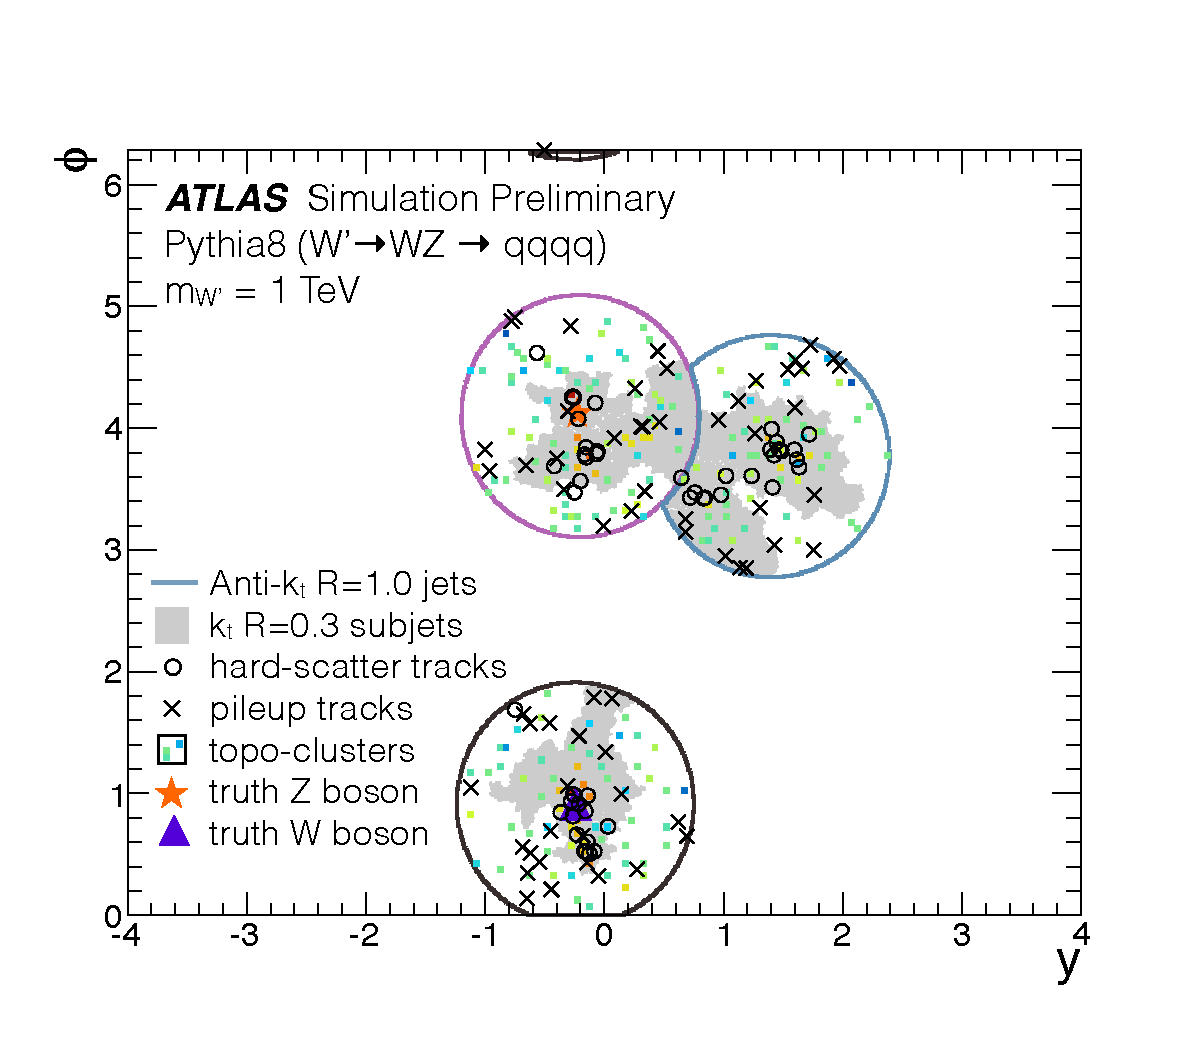
\includegraphics[width=0.6\textwidth]{fig_20a.pdf}
\label{fig:jet-reconstruction:pu_subjet}
\caption{An example of a jet contaminated by a pileup subjet (i.e., the \largeR jet with the truth $Z$-boson).}
\end{figure}

%%%%%%%%%%%%%%%% 
\section{Flavor Tagging}

Another important aspect of jet reconstruction is the \textit{flavor tagging} of jets.  This refers to the identification of a long-lived (typically $\tau \approx 1.5$~ps) $B$-hadrons within jets, and so is commonly also called $b$-tagging. $B$-hadrons, because of this comparatively long life time (long, compared to the $10^{-20}$~s lifetimes of the $W$ or $Z$, for example) and the relativistic time dilation at high energy, decay at macroscopic distances (typically a few mm) away from the primary vertex in the transverse direction at a location referred to as a \textit{secondary vertex}. Precision tracking detectors are able to identify these displaced tracks and vertices, allowing $B$-jets to be identified against very large light-flavor backgrounds. As interesting physics signatures-- SUSY, top decays, Higgs decays, and so on-- often involve final states with $b$-jets, the identification of such jets is critical to the physics program of the LHC~\cite{ATLAS-B}.

There are many different complementary techniques used to identify $B$-hadrons~\cite{ATLAS-B}. The following is a description of the most important techniques, and their comparative advantages. All the algorithms share a common baseline track association, which uses a \pt-dependent $\Delta R$ cone of maximum size $R=0.45$ at $\pt = 20$~GeV and $R=0.25$ at $\pt = 150$~GeV. The actual tracks selected are tuned in detail to keep the best tracks for each algorithm; the restrictions on some include a requirement on the $B$-layer of the pixel detector or not, varying \pt tresholds (either 400 MeV and 1 GeV), and the rejection of two-track vertices with mass consistent with the decay or conversion of a $\gamma$, $K$, or $\Lambda$.

\subsection{IP3D}

The simplest of the main ATLAS $b$-taggers, IP3D searches for tracks with significant impact parameters, which are therefore inconsistent with originating from the primary vertex~\cite{ATLAS-B}. Both the longitudinal ($z_0$) and transverse ($d_0$) impact parameters are measured, and a significance is calculated by dividing each distance by the estimated error on the measurement, and so well measured tracks are weighted more highly than poorly measured tracks. The sign of the impact parameter is also used: a positive sign indicates that the track extrapolation crosses the direction of the jet in front of the primary vertex and is consistent with the decay of a long-lived particle moving transversely from the primary vertex. Tracks from light-flavor decays can be mismeasured and appear in front of and behind the jet equally; thus, selecting jets with the tracks in front (i.e., with positive significance) can reduce light-flavor backgrounds. Figure~\ref{fig:jet-reconstruction:b-tagging:ip3d} shows each of these variables in dijet data and MC from early data collected in 2011. The information from both of these variables is combined in a likelihood to create the output of IP3D, also displayed in Figure~\ref{fig:jet-reconstruction:b-tagging:ip3d}.

%%%%%%%%%%%%%%%%%%%%%

\begin{figure}
\centering
\subfigure[$d_0$, the transverse impact parameter]{\includegraphics[width=0.3\textwidth]{fig_03}}
\subfigure[$z_0$, the longitudinal impact parameter]{\includegraphics[width=0.3\textwidth]{fig_04}}
\subfigure[Combined IP3D weight]{\includegraphics[width=0.3\textwidth]{fig_07}}
\label{fig:jet-reconstruction:b-tagging:ip3d}
\caption{Distribution of the signed impact parameter significances used by the IP3D tagging algorithm, and the combined IP3D output, in a dijet sample in both data and MC.}
\end{figure}

%%%%%%%%%%%%%%%%%%%%%

%The sign is positive if the track extrapolation crosses the jet direction in front of the primary vertex, and negative otherwise.

\subsection{SV1}

The SV1 algorithm, as the named suggests, uses information about the secondary vertex reconstruction in the jet~\cite{ATLAS-B}. Two separate vertexing approaches are used: first, all two-track vertices are considered, with pairs rejected if they are consistent with a material interaction or decay of some non-$B$-hadron. The number of these remaining vertices is used as a discriminating variable: $b$-jets are expected to have a higher number than light-flavor jets. Additionally, all the tracks from the surviving two-track vertices are combined to form an inclusive secondary vertex, which aims to reconstruct the true decay location of the $B$-hadron (though it also includes the decay of any subsequent $D$-hadrons, which may also be somewhat displaced). Tracks are iteratively removed from this secondary vertex until a $\chi^2$ goodness of fit threshhold is reached. The energy and mass of the remaining tracks associated to the secondary vertex are combined in a likelihood and used as a discriminating variable. The 3D displacement significance of this vertex, $L_{\mathrm{3D}} / \sigma_{L_\mathrm{3D}}$, is the primary variable used to discriminate between light-flavor and $b$-jets. Finally, the $\Delta R$ between the direction of the jet and the secondary vertex is used as an additional discriminating variable. Several of these variables are displayed in Figure~\ref{fig:jet-reconstruction:b-tagging:sv1}. 

%%%%%%%%%%%%%%%%%%%%%

\begin{figure}
\centering
\subfigure[SV mass]{\includegraphics[width=0.3\textwidth]{fig_10a_sv1}}
\subfigure[SV energy fraction]{\includegraphics[width=0.3\textwidth]{fig_10b_sv1}}
\subfigure[Number of two-track vertices]{\includegraphics[width=0.3\textwidth]{fig_10c_sv1}}
\label{fig:jet-reconstruction:b-tagging:sv1}
\caption{Several of the inputs used in the SV1 $b$-tagging algorithm, in a dijet sample in both data and MC.}
\end{figure}

%%%%%%%%%%%%%%%%%%%%%

\subsection{JetFitter}

The JetFitter algorithm is the most sophisticated of the standalone taggers~\cite{ATLAS-B,JetFitter}, and targets the separate reconstruction of the $B$- and $D$-hadron decay vertices. Using a Kalman filter technique, tracks associated to a jet iteratively update the location of the primary vertex, the $B$-hadron flight direction, and the distance between the $B$ flight direction and the track. Each intersection of the track with the flight direction is a potential secondary vertex; pairs determined to be close to each other, and likely to be part of the same physical vertex, are then iteratively merged. The result, which typically leads to two reconstructed, in-line vertices (corresponding to the $B$ and $D$ decays), can be used as a tagger. A likelihood (binned in the number of tracks and vertices into 13 orthogonal categories) is formed using several pieces of information from each vertex: the mass of the tracks, the energy fraction of the tracks compared to the energy of the jet, and the weighted decay length significance. Figure~\ref{fig:jet-reconstruction:b-tagging:jetfitter} shows several of these input variables, and Figure~\ref{fig:jet-reconstruction:b-tagging:jetfitter_total} shows the output of the JetFitter likelihood.

%%%%%%%%%%%%%%%%%%%%%

\begin{figure}
\centering
\subfigure[Number of 2-track vertices]{\includegraphics[width=0.3\textwidth]{fig_16a}}
\subfigure[Decay chain mass]{\includegraphics[width=0.3\textwidth]{fig_16c}}
\subfigure[Decay chain energy fraction]{\includegraphics[width=0.3\textwidth]{fig_16d}}
\label{fig:jet-reconstruction:b-tagging:jetfitter}
\caption{Several of the inputs used in the JetFitter $b$-tagging algorithm, in a dijet sample in both data and MC.}
\end{figure}

%%%%%%%%%%%%%%%%%%%%%


%%%%%%%%%%%%%%%%

\begin{figure}
\centering
\includegraphics[width=0.6\textwidth]{fig_14.pdf}
\label{fig:jet-reconstruction:b-tagging:jetfitter_total}
\caption{The output of the JetFitter $b$-tagging likelihood, in a dijet sample in both data and MC.}
\end{figure}

%%%%%%%%%%%%%%%% 

\subsection{MV1}

Each of these algorithms contains useful orthogonal information, and the most performant approach to $b$-tagging combines all of them. A neural network is used to combine the outputs of IP3D, SV1, and JetFitterCombNN (itself the output of a neural network combining IP3D and JetFitter), producing a variable called MV1~\cite{ATLAS-B-Eff}\footnote{The use of both IP3D separately, in combination in the JetFitterCombNN variable, is not optimal in the construction of a multivariate algorithm, but in principle the correlations can be properly measured and accounted for by the neural network}. Figure~\ref{fig:jet-reconstruction:b-tagging:mv1} shows the $b$-jet efficiency vs light jet rejection in MC; the improvement of the MV1 algorithm over the other taggers is substantial.

%%%%%%%%%%%%%%%%

\begin{figure}
\centering
\includegraphics[width=0.6\textwidth]{fig_01a.pdf}
\label{fig:jet-reconstruction:b-tagging:mv1}
\caption{A comparison, using $t\bar{t}$ MC, of the $b$-jet efficiency vs. light jet rejection of several $b$-tagging algorithms.}
\end{figure}

%%%%%%%%%%%%%%%% 

\subsection{Calibration}
\label{chapter:jet-reconstruction:b-tagging:calibration}
After $b$-tagging algorithms are developed, they also need to be \textit{calibrated} in data in order to be useful for physics analyses. The algorithms are all trained in simulation, and have some dependence on the hadronization and fragmentation modeling of these MC generators: for this reason, the outputs of the algorithms can differ in data and MC (as seen in the previous figures), and so the efficiency of $b$-tagging (on both $b$ and light jets) can also differ in data and MC~\cite{ATLAS-B-Eff,ATLAS-B-Eff-Mistag,ATLAS-B-Eff-LL,ATLAS-B-CL}. Many techniques are used to measure the efficiency in data (and derive the corresponding scale-factors to adjust MC to data), and determine the systematic uncertainties on these efficiencies. The scale factors are typically close to 1, and uncertainties are typically near 10\%, as shown in Figure~\ref{fig:jet-reconstruction:b-tagging:calib}.

%%%%%%%%%%%%%%%%

\begin{figure}
\centering
\includegraphics[width=0.6\textwidth]{fig_02b-2}
\label{fig:jet-reconstruction:b-tagging:calib}
\caption{The size of the scale factor for $b$-tagging calibration in data, as a function of the jet \pt, and the size of the corresponding uncertainties.}
\end{figure}

%%%%%%%%%%%%%%%% 

\section{Quark/Gluon Discrimination}
\label{jet-reconstruction:qg}
\subsection{Overview}
\label{jet-reconstruction:qg:overview}
%~\cite{Miyazawa:1966,Ramond:1971gb,Golfand:1971iw,Neveu:1971rx,Neveu:1971iv,Gervais:1971ji,Volkov:1973ix,Wess:1973kz,Wess:1974tw}

Just as $b$-tagging is useful for search for new physics in channels with heavy flavor, the identification of \textit{light quarks} can also be important when searching for new physics. Most commonly, the jets associated with multi-jet production arise from gluon radiation, and so a tool to eliminate these backgrounds can be very useful. Even searches for the Higgs boson decaying to hadronic $W$-bosons or $Z$-bosons can benefit, as once again the signal is dominated by light-quark jets and backgrounds are often gluon-induced.

This type of discrimination has been attempted at several experiments before ATLAS~\cite{TevatronShapes1,QGNN,Pumplin,QGopal,Ariel,QGsub,QGlep,QGcleo,DelphiQG,DelphiQG2,AlephQG,L3QG}. This discrimination tends to rely on the different color charges for quarks ($C_F=4/3$) and gluons ($C_A=3$), which leads to a leading order prediction that gluon jets have $C_A/C_F = 9/4$ more particles (which are consequently more widely distributed, and generally softer) than light-quark jets. OPAL's measurement~\cite{QGopal} indeed measured something very similar to this prediction. Because of their much simpler experimental environments, experiments like OPAL at $e^+/e^-$ colliders have generally been much more successful at discriminating between quarks and gluons, as determining ``pure'' samples at a hadron collider is exceedingly difficult. However, recent developments from the theory communited have suggested not just that pure samples suitable for calibration are obtainable, but also that discrimination is possible in the challenging underlying-event and pileup heavy environment of a hadron collider~\cite{schwartz1,schwartz2}. \editnote{Some of these citations need to be cleaned up}

This section follows the results of the ATLAS paper on quark-gluon discrimination using 2011 data~\cite{ATLASqg}. First, quark and gluon jets are more precisely defined, followed by a description of possible discriminating variables. The use of data-driven templates is discussed, and then the final tagger properties and power is presented.

\subsection{Definition of Light Quark and Gluon Jets}
\label{jet-reconstruction:qg:definition}

The labeling of a $b$-jet or a $c$-jet is a fairly straightforward process: the initiating $b$ and $c$ quarks, though unmeasurable and therefore un-physical themselves, inevitably hadronize into observable $B$ and $D$ hadrons. Thus, the presence of a $B$ or $D$ hadron, at the MC simulation level, is enough to provide a label to the jet: if a $B$ or $D$ hadron is present, it is clear that a secondary vertex can occur, and the jet should be counted as being heavy-flavor.

This unambiguous hadronization does not occur for light-quark and gluon jets. In the parton shower process, gluons even split into pairs of quarks before hadronization: all gluon jets contain quarks, in some sense. Moreover, the observable particles-- kaons, pions, protons, neutrons, and so on-- are all identical for quark and gluon initiated jets. Even before attempting discrimination between the two classes, then, it is difficult to precisely state what we are discriminating between.

One potentially less ambiguous definition is to use the partons from the matrix element to label jets. This has the disadvantage that only some jets can be labelled-- in particular, in multi-jet events, depending on the generator, as few as 2 partons are simulated as part of the matrix element, and therefor only two jets out of many could be labelled. A better strategy is to simply use the highest energy parton within $\Delta R < R_\mathrm{jet}$ of the jet. When studied with both Pythia $2\rightarrow2$ and MadGraph $2\rightarrow4$ generators, this matching followed the labelling from the matrix element in $> 95\%$ of events. This labelling has the advantage of also working on the hadronic decays of top quarks or $Z$-bosons. For the rest of the discussions in this section, this labeling scheme will be implied when discussing quark and gluon jets.

While this analysis does not directly attempt to tag $b$ and $c$ jets, they must often be subtracted from the samples in order to deal with only light-flavor jets. These jets are labelled with the following priority: if a $B$-hadron with $\pt > 5$ GeV exists within $\Delta R < R_\mathrm{jet}$, label it a $b$-jet. If two such independent hadrons exist, label it a $bb$ jet (originating from a gluon splitting, but not considered in this analysis). If this fails, search for a $D$-hadron with $\pt > 5$ GeV within the jet; if one is found, label it a $c$-jet, and if two are found, label it $cc$. Only after these steps have determined that there are no heavy flavor quarks within the jet is the jet's light-flavor type assessed.

\subsection{Data and MC Samples}
\label{jet-reconstruction:qg:samples}

Several different data and MC samples are used to study the properties of quark and gluon jets. There are two main categories: multi-jet and $\gamma$+jet events. 

Multi-jet events are modelled by Pythia 6 and \texttt{Herwig++} simulation, and some smaller samples using Madgraph interfaced with Pythia 8. Events are selected in data with single jet triggers with various thresholds which are fully efficient at $\pt > 40$~GeV. The lower \pt threshhold triggers are \textit{prescaled} to reduce the rate at high luminosity. When binning results in \pt, each bin is filled exclusively with events from a single trigger that is fully efficient in that range (and the second jet is used only if its \pt also is in this same bin). When studying tri-jet events, the same \pt binning and trigger treshholds are used.

The $\gamma$+jet sample is selected with single photon triggers, again with variable tresholds and corresponding prescales. The lowest threshold is at $p_\mathrm{T}^\gamma > 25$~GeV, and a back-to-back requirement between the $\gamma$ and jet, $\Delta \phi > 2.8$, is imposed. An additional veto on soft radiation is imposed, wherein the uncalibrated \pt of the sub-leading jet is required to be less than $30\%$ of $p_\mathrm{T}^\gamma$~\cite{JES2010}\footnote{In the corresponding 2012 analysis, it was discovered that this cut changes the \pt distribution within each \pt bin and slightly biases the result, lowering slightly the performance of the tagger.}. Each jet \pt bin is filled by a single-photon trigger that is fully efficient in that bin, as the balance between photon and jet guarantees. The same triggers are used in the $\gamma$+2jet sample, except that the subleading jet \pt cut is removed.

% The dijet sample is selected using single-jet triggers with various thresholds [48], which are fully efficient for jets with pT > 40 GeV. Each jet pT bin is filled exclusively by a single trigger that is fully efficient for jets in that pT range, following Ref. [1]. The trijet sample uses the same trigger selection as the dijet sample. This guarantees that studies using the jet with the third highest pT in each event are not biased by the trigger.

%The γ+jet sample is selected using single-photon trig-gers. The lowest threshold single-photon trigger is fully efficient for photons with pT > 25 GeV. For this sam- ple, a back-to-back requirement for the photon and the leading jet, ∆φ > 2.8, is imposed. An additional veto on soft radiation is also applied to further reduce back- ground contamination [41]: the uncalibrated pT of the sub-leading jet is required to be less than 30% of the photon pT. Relying on the pT balance of the photon and jet, each jet pT bin is filled exclusively by a single-photon trigger that provides a fully efficient selection.
%The same triggers are used in the γ+2-jet sample in each region of jet pT. Since the sub-leading jet pT is lower than that of the leading jet by definition, this selection is also not biased by jet reconstruction effects.

\subsection{Quark and Gluon Jet Properties}
\label{jet-reconstruction:qg:properties}

Given the expectations developed in Section~\ref{jet-reconstruction:qg:overview}, there are many different jet observables which could potentially distinguish between quark and gluon initiated jets. One approach is to try to measure the number of particles to take advantage of the color factor difference. In principle, a variable just as $n_\mathrm{clusters}$ would be ideal, as it is expected to be directly proportional to the number of stable particles interacting with the calorimeter. However, as the granularity of the calorimeter changes with $\eta$, and the number of clusters grows unbounded with pileup, this is not a very useful variable. A related alternative is \ntrk, the number of tracks associated to a jet\footnote{Note that in this analysis, tracks are associated with a $\Delta R < R_\mathrm{jet}$ requirement instead of a ghost association. As most jets considered are isolated, and \antikt~is used throughout, this is a reasonable simplification.}. This is expected to have much less $\eta$ dependence, and because tracks from pileup vertices are able to be rejected, is stable with regards to the amount of pileup.

Other variables take into account the radial distribution of the energy inside the jet. One simple such variable is the \textit{jet width}, as discussed in Section~\ref{jet-reconstruction:calibration:gsc}. The width is the first radial moment of the \pt of the jet: jets with a very focused core will have lower width, and jets with a more even distribution of energy will have a higher width. Gluons, because they first split to quarks, and because of their higher color factor, are expected to have broader energy distributions and therefore higher width. The width can be calculated with clusters as inputs, or the tracks associated to a jet. Because of the issues with pileup, track width is used in this analysis.

Many other variables, as documented in \cite{schwartz1}, are possible, but these two were the preferred combination from early theoretical studies. Another set of studies~\cite{EEC} indicated that a new observable, the energy-energy correlated angularity, could also be useful. This class of observables is defined as:
\begin{equation}
{\rm ang_{\rm EEC}}=\frac{ \sum_i \sum_j p_{{\rm T},i} \times p_{{\rm T},j} \times (\Delta R(i,j))^\beta}{ (\sum_i p_{{\rm T},i})^2 },
\end{equation}
where $i$ runs over the tracks associated to the jet and $j$ runs over the tracks associated to the jet with $j>i$ (the calorimeter version is sensitive to pileup, and therefore not studied), and $\beta$ is a tunable parameter typically $O(1)$. While this variable is in principle very sensitive, several effects conspire to limit its effectiveness and prevent it from being used in the final result (as will be discussed shortly).

To characterize the separation between quark and gluon jets with these variables, we define the \textit{separation} as~\cite{2006physics11219P}:
%
\begin{equation}
s=\frac{1}{2}\int\frac{(p_q(x)-p_g(x))^2}{p_q(x)+p_g(x)}dx = \frac{1}{2}\sum_i\frac{(p_{q,i}-p_{g,i})^2}{p_{q,i}+p_{g,i}}, 
\label{eq:separation}
\end{equation}
%
where $i$ runs over bins of a histogram. This is a measure of the overlap of two distributions, $q(x)$ and $g(x)$, which are the quark and gluon distributions respectively in a Pythia dijet simulation.  The result is shown in Figure~\ref{fig:jet-reconstruction:qg:separation}: in general, the separation power increases as a function of \pt, and \ntrk is predicted to have the best power. Track width performs worse than many of the other variables, but because of its resilience in modeling (compared to the EEC variables) and its robustness to pileup (compared to the calorimeter width), it will also be studied further. Moreover, the track width has a very low correlation with \ntrk: as low as $15\%$ at low \pt and only $50\%$ at high \pt, whereas the EEC variables have consistent correlations of $75\%$. This means that a combined observable from \ntrk and track width will likely outperform other options.

%%%%%%%%%%%%%%%%

\begin{figure}
\centering
\includegraphics[width=0.6\textwidth]{qg/SeparationPower}
\label{fig:jet-reconstruction:qg:separation}
\caption{The size of the scale factor for $b$-tagging calibration in data, as a function of the jet \pt, and the size of the corresponding uncertainties.}
\end{figure}

%%%%%%%%%%%%%%%% 

\subsection{Data-Driven Templates}

Figures~\ref{fig:jet-reconstruction:qg:dijetProperties} and \ref{fig:jet-reconstruction:qg:gammajetProperties} show the \ntrk and Track Width distributions for data, \Pythia, and \Herwigpp generators, in both dijet and $\gamma$+jet topologies. The distributions show that while there is decent agreement for the width, the \ntrk variable is very poorly modelled: \Pythia predicts too many tracks consistently, while \Herwigpp predicts too few. 

\begin{figure}[tbp]
\begin{center}
\subfigure[]{
\includegraphics[width=0.48\textwidth]{qg/dijetakt4TopoEM_ntrk_PT60_eta0.pdf}
}
\subfigure[]{
\includegraphics[width=0.48\textwidth]{qg/dijetakt4TopoEM_ntrk_PT260_eta0.pdf}
} \\
\subfigure[]{
\includegraphics[width=0.48\textwidth]{qg/dijetakt4TopoEM_trkwidth_PT60_eta0.pdf}
}
\subfigure[]{
\includegraphics[width=0.48\textwidth]{qg/dijetakt4TopoEM_trkwidth_PT260_eta0.pdf}
}
\caption{
Jet \ntrk (top) and track width (bottom) for jets with $60<\pt<80$~\GeV\ (left) and
$260<\pt<310$~\GeV\ (right) in {\sc Pythia} 6, {\sc Herwig++}, and data, for a dijet selection.
Jets have $|\eta|<0.8$ and are reconstructed with an \AKT\ jet algorithm with $R=0.4$.
 }
\label{fig:jet-reconstruction:qg:dijetProperties}
\end{center}
\end{figure}

\begin{figure}[tbp]
\begin{center}
\subfigure[]{
\includegraphics[width=0.48\textwidth]{qg/gammaakt4TopoEM_ntrk_PT60_eta0.pdf}
}
\subfigure[]{
\includegraphics[width=0.48\textwidth]{qg/gammaakt4TopoEM_ntrk_PT260_eta0.pdf}
} \\
\subfigure[]{
\includegraphics[width=0.48\textwidth]{qg/gammaakt4TopoEM_trkwidth_PT60_eta0.pdf}
}
\subfigure[]{
\includegraphics[width=0.48\textwidth]{qg/gammaakt4TopoEM_trkwidth_PT260_eta0.pdf}
}
\caption{
Jet \ntrk (top) and track width (bottom) for jets with $60<\pt<80$~\GeV\ (left) and
$260<\pt<310$~\GeV\ (right) in {\sc Pythia} 6, {\sc Herwig++}, and data, for a $\gamma+$jet selection.
Jets have $|\eta|<0.8$ and are reconstructed with an \AKT\ jet algorithm with $R=0.4$.
 }
\label{fig:jet-reconstruction:qg:gammajetProperties}
\end{center}
\end{figure}

This makes the usual prospect of constructing a tagger-- beginning with a likelihood trained in MC and calibrating small residual differences in data-- a challenging prospect. Instead, we first extract a pure quark or gluon shape from data, and construct the tagger from these shapes. To construct these shapes, we look at histograms in two different samples, where we can measure the quark/gluon flavor fraction very precisely using the matrix element of the generator\footnote{And while generator hadronization properties vary greatly, this fraction of quark and gluon jets is rather consistent; any residual difference, at the $10\%$ level, is taken as a systematic later in the procedure.}. For each bin $i$ of jet $\eta$, jet $\pt$, and jet property (track width, number of tracks, or the two-dimensional distribution of the these), a set of linear equations is solved:
%
\begin{align}
P_i(\eta,\pt) &= f_{q}(\eta,\pt) \times P_{q,i}(\eta,\pt) \nonumber \\
	& + f_{g}(\eta,\pt) \times P_{g,i}(\eta,\pt) \nonumber \\
& + f_{c}(\eta,\pt) \times P_{c,i}(\eta,\pt) \nonumber \\
& + f_{b}(\eta,\pt) \times P_{b,i}(\eta,\pt) , 
\label{eq:fractions}
\end{align}
%
where $P_i$ is the value of the relevant distribution in bin $i$ of the distribution in the dijet
or $\gamma+$jet sample, $f_{q}$ and $f_{g}$ are the light-quark and gluon fractions 
predicted by \Pythia at a given $\eta$ and $\pt$, 
and $P_{q,i}$ and $P_{g,i}$ are the values of the relevant distribution 
for quark- and gluon-jets in bin $i$ of the distribution. The fractions 
$f_{c}$ and $f_{b}$ for $c$-jets and $b$-jets are relatively small. They are taken from the
MC simulation, together with the corresponding distributions $P_{c}$ and $P_{b}$.
The same is true for the fractions and distributions for $g\rightarrow c\bar{c}$ and $g\rightarrow b\bar{b}$,
not shown in Eq.~\ref{eq:fractions} for brevity. The heavy flavor fractions are typically below $5-10\%$, and are taken directly from MC and subtracted from the distributions.

This leaves two equations (one for a dijet sample, and one for $\gamma$+jet), with two unknowns ($P_{q}$ and $P_{g}$), which can be solved bin-by-bin. The only MC input is from the fractions-- the rest of the shape of the resulting distribution comes from data. The studies are performed in three bins of $|\eta|$: $|\eta|<0.8$, $0.8<|\eta|<1.2$ and $1.2<|\eta|<2.1$, though in general only the results from the central bin will be shown for the sake of brevity. Note that this technique depends on the assumption that the shape of a quark jet in a $\gamma$+jet sample is the same as that of a quark jet in a dijet sample: as we will later see, this is largely true, but residual differences will account for the largest systematic. An additional fake term,  $f_{{\rm fake}, i}(\eta,\pt)\times P_{{\rm fake}, i}(\eta,\pt)$, is added to the distributions in the $\gamma$+jet sample to take into account the fake photons which contaminate this sample~\cite{JES2011}.

This method is first tested for the individual distributions of \ntrk and Track Width in MC, as in the top subfigures of Figure~\ref{fig:jet-reconstruction:qg:ntrkWidthClos}. The closure in \Pythia is very good: the small residual differences between the extracted templates and the inputs are taken as a systematic later. The dijet sample, as it contains more gluons, is in some sense the basis of the gluon distribution; likewise, as the $\gamma$ is more likely to radiate from a charged object than a neutral, the $\gamma$+jet sample is more quark-enriched and the extraction leads to a quarks following the $\gamma$+jet sample more closely. With the technique validated in MC, we can also use it in data, replacing the relevant value from data into the $P_i$ of Equation~\ref{eq:fractions}. The results of this are shown in Figure~\ref{fig:jet-reconstruction:qg:ntrkWidthClos} in the bottom panel: we see now a confirmation of the earlier studies, in that the \ntrk variable is clearly poorly modelled by the MC. In particular, the \textit{gluon} distribution is strongly incorrect for \ntrk, while quarks fare better; the Track Width distribution is reasonably well modelled for both quarks and gluons, as expected. As the differences between data and MC make quarks and gluons more similar than predicted by the simulation, we can expect a degraded tagger performance compared to the naive expectation.


\begin{figure*}[p]
\begin{center}
%Subfigures
\subfigure[]{
\includegraphics[width=0.45\textwidth]{qg/ntrk_akt4TopoEM_eta0_means_withMCin_FromMC_Pyth}
}
\subfigure[]{
\includegraphics[width=0.45\textwidth]{qg/trkwidth_akt4TopoEM_eta0_means_withMCin_FromMC_Pyth}
} \\
\subfigure[]{
\includegraphics[width=0.45\textwidth]{qg/ntrk_akt4TopoEM_eta0_means_withMCin}
}
\subfigure[]{
\includegraphics[width=0.45\textwidth]{qg/trkwidth_akt4TopoEM_eta0_means_withMCin}
}
\caption{ Average (a,c) \ntrk and (b,d) track width for quark- (solid symbols) and gluon-jets
(open symbols) as a function of reconstructed jet $\pt$ for isolated jets with $|\eta|<0.8$.
Results are shown for distributions obtained using the in-situ extraction method in
\Pythia 6 simulation (black circles, (a,b)) or data (black circles, (c,d)), as well as for 
labeled jets in the dijet sample (triangles) and in the $\gamma$+jet sample (squares).
The error bars represent only statistical uncertainties. Isolated jets are reconstructed using the
\akt jet algorithm with radius parameter $R=0.4$. The bottom panels show
the ratio of the results obtained with the in-situ extraction method to the results
in the dijet and $\gamma$+jet MC samples. }
\label{fig:jet-reconstruction:qg:ntrkWidthClos}
\end{center}
\end{figure*}

There are several sources of uncertainty in the extraction procedure:

\begin{enumerate}
\item Uncertainties on input fractions ($f_{x,i}$)
\item Uncertainties on the input shapes ($P_{x,i}$) 
\item Uncertainties on the fake photon background
\item Sample dependent effects (the differences between quarks in $\gamma$+jet and dijet samples)
\end{enumerate}

The input fraction uncertainties are addressed by comparing the fractions in \Pythia and MadGraph, and taking the difference as directly as a systematic. This takes into account differences potentially due to different renormalization/factorization scales, and the different ways of simulating the emission of quarks/gluons. A $5\%$ uncertainty, anti-correlated between the quark and gluon fractions, is assigned as a conservative systematic. The differences due to the mismodelling of the PDF is also included as a systematic. A combination of different PDF sets are assessed, each with different properties. They use different fitting procedures (MRST, CTEQ, and NNPDF), and are accurate to different orders in the perturabtive expansion (MSTW2008lo for LO, CT10 for NLO), and have different assumptions about the $\alpha_s$ calculation (MRST2007lmod for LO$^*$ and MRSTMCal for LO$^{**}$). Another $5\%$ anti-correlated systematic takes these effects into account conservatively.

Uncertainties on the shapes come from the MC dependence on the $b$ and $c$-jet shapes. Uncertainties on the $b$-jet shapes are determined from a $t\bar{t}$ sample with $> 95\%$ purity: a $10\%$ systematic is assigned on the $b$-jet properties to take this into account. For $c$-jets, templates with 10\% increases in the rates of 2-prong, 3-prong, and 4-prong decays are used to estimate the effect of changes to the $c$-hadron decay. The largest propagated difference of these is used as the systematic uncertainty on the tagger.

The fake photon background is assessed in several ways. The fake-factors are developed using an ABCD procedure, and the cuts used to define each of the regions are varied to assess the sensitivity to these effects. This results in a purity difference of $10\%$ for low \pt jets, and is the dominant uncertainty related to the photon measurement.

The sample dependent uncertainty is the largest, and takes into account the differences in the MC's seen in Figure~\ref{fig:jet-reconstruction:qg:ntrkWidthClos}. 
Uncertainties on the jet properties are estimated first from differences
between the $\gamma+$jet and dijet samples of the properties of quark- and gluon-jets, using both \Pythia and \Herwigpp. The envelope of these
variations is used to estimate a systematic uncertainty, but is prone to large fluctuations due to the limited statistics of the MC samples. These statistical 
uncertainties
are estimated and used to smooth the $\pt$ dependence of the uncertainty following the
procedure described in \cite{JES2011}: a Gaussian kernel with size proportional to the inverse of the uncertainty averages over the \pt bins, weighting those with lower statistical uncertainty higher. 
The sample dependence is consistently the dominant systematic uncertainty for all jet $\pt$, and thus it is critical to take into account these variations.

\subsection{Validation with event-level kinematic cuts}
\label{jet-reconstruction:qg:validation}

While the shapes derived in the previous section are data-driven, the large data and MC differences motivate an independent check in completely separate samples for the purpose of validation. Luckily, \cite{schwartz2} proposed several samples, accessible at hadron colliders, with quark/gluon purity of $> 90\%$ which could be used for validation purposes. These samples are very statistically limited and therefore insufficient to determine the shapes used for a tagger themselves, but can serve very well as test samples. Moreover, these independent samples give a feeling for any residual color-flow or event-level dependence which the previous uncertainty procedure may have missed.

Gluon jets are found in the dijet sample, particularly because the proton have a very large gluon component at low $x$. However, as \pt rises, the gluon fraction falls off rapidly, leaving a mixed sample when measured at any appreciable \pt. In multi-jet events, however, any radiated jet is relatively more likely to originate from a gluon. As this radiation is likely to be soft, the third-leading jet is thus more likely to be a gluon. A kinematic discriminant, using only information on the relative location of jets, can further purify the tri-jet sample: 
%
\begin{equation}
\zeta=|\eta_3|-|\eta_1-\eta_2|,
\end{equation}
%
where $\eta_i$ is the pseudorapidity of the $i$th leading jet. Cutting on $\zeta < 0$ results in a tri-jet sample with gluon purity $> 90\%$, as determined in MadGraph simulation. To evaluate the determination of the gluon shapes from Figure~\ref{fig:jet-reconstruction:qg:ntrkWidthClos}, those templates are directly compared to the sample with $\zeta < 0$. This comparison is presented in \ref{fig:jet-reconstruction:qg:pure_trijet_ntrkTrkWidth1} and \ref{fig:jet-reconstruction:qg:pure_trijet_ntrkTrkWidth2} of Figure~\ref{fig:jet-reconstruction:qg:pure_trijet_ntrkTrkWidth}. The agreement between the extracted template and the completely independent pure data sample of gluons is very good, for both \ntrk and Track Width. In particular, the \ntrk distributions agree quite well, and the purified sample agrees better with the data than the \Pythia simulation.

\begin{figure}[p]
\begin{center}
\subfigure[]{
\label{fig:jet-reconstruction:qg:pure_trijet_ntrkTrkWidth1}
\includegraphics[width=0.45\textwidth]{/qg/smoothed_ntrk_akt4TopoEM_eta0_PureExtractedG}
}
\subfigure[]{
\label{fig:jet-reconstruction:qg:pure_trijet_ntrkTrkWidth2}
\includegraphics[width=0.45\textwidth]{qg/smoothed_trkwidth_akt4TopoEM_eta0_PureExtractedG}
} \\
\subfigure[]{
\label{fig:jet-reconstruction:qg:pure_trijet_ntrkTrkWidth3}
\includegraphics[width=0.45\textwidth]{qg/smoothed_ntrk_akt4TopoEM_eta0_PureExtractedQ}
}
\subfigure[]{
\label{fig:jet-reconstruction:qg:pure_trijet_ntrkTrkWidth4}
\includegraphics[width=0.45\textwidth]{qg/smoothed_trkwidth_akt4TopoEM_eta0_PureExtractedQ}
}
\caption{Top, the jet (a) \ntrk and (b) track width as a function of $\pt$ for jets in a
gluon-jet-enriched trijet sample (triangles) compared to gluon-jet extracted templates (circles) for
$|\eta|<0.8$. Bottom, the jet (c) \ntrk and (d) track width as a function of $\pt$ for jets in a quark-jet-enriched $\gamma$+jet
sample (triangles) compared to quark-jet extracted templates (circles) for jets with $|\eta|<0.8$.
Jets are reconstructed with the \antikt algorithm with $R=0.4$. The bottom
panels of the figures show the ratios of the results found in the enriched sample to the extracted
results. Error bars on
the points for the enriched sample correspond to statistical uncertainties. The inner
shaded band around the circles and in the ratio represents statistical uncertainties on the
extracted results, while the outer error band represents the combined systematic and statistical
uncertainties.
}
\label{fig:jet-reconstruction:qg:pure_trijet_ntrkTrkWidth}
\end{center}
\end{figure}

Events with photons are already used to extract the more quark-like component of the templates: events with one jet and one photon have $>80\%$ quark purity at $\pt > 150$~GeV. Enrichment of this sample is difficult, and anyway, we have already used it for the template extraction and so validation requires a new sample. A sample with a single photon and two jets turns out to be more effective~\cite{schwartz2}: if no additional selection is applied, they have a lower purity, but another kinematic event-level cut can be used to significantly purify the sample by helping to identify the jets seeded by the parton that is most likely to have radiated the photon (which is more likely to be a quark because the photon requires electric charge to be radiated). The observable is defined as:
%
\begin{equation}
\xi=\eta_\text{jet~1}\times\eta_\gamma+\Delta R_{(\text{jet~2},\gamma)},
\end{equation}
%
where $\eta_\gamma$ ($\eta_\text{jet~1}$) is the $\eta$ of the photon (leading jet), and 
$\Delta R_{(\text{jet~2},\gamma)}$ gives the difference in $\eta$--$\phi$ space between the sub-leading 
jet and the photon. By imposing a requirement on this variable of $\xi < 1$, purities over 90\% can be achieved (as validated with MadGraph siulation), although with a significant loss of events. This sample can again be compared to the extracted templates for quarks from Figure~\ref{fig:jet-reconstruction:qg:ntrkWidthClos}. This comparison is presented in \ref{fig:jet-reconstruction:qg:pure_trijet_ntrkTrkWidth3} and \ref{fig:jet-reconstruction:qg:pure_trijet_ntrkTrkWidth4} of Figure~\ref{fig:jet-reconstruction:qg:pure_trijet_ntrkTrkWidth}. Once again, the agreement between the independent data sample and the extracted templates is very good for both the \ntrk and Track Width variables, validating our use of our templates for both quark and gluon jets.

\subsection{Creating a Tagger, and Results}

As the discriminating power of Track Width and \ntrk changes with \pt (\ntrk gains power as \pt rises, while the opposite is true for Track Width), a combined likelihood between the two variables will be the most effective tool for quark-jet tagging\footnote{Though a gluon jet tagger is also possible, the details are not considered in this analysis.}. Such a likelihood is defined using the normalized extracted two-dimensional distributions (called $q$ and $g$),
%
\begin{equation}
L=\frac{q}{q+g}.
\end{equation}
%
A cut on this variable $L$, built in bins of \pt and $\eta$, will effectively discriminate between quarks and gluons. Note that the two-dimensional distributions are first smoothed with a Gaussian kernel and dynamically rebinned to ensure that all regions of the distributions are populated sufficiently\footnote{In particular, low statistics in the $q$ distribution also causes a rebinning of the $g$ distribution, in order to make the likelihood construction as simple as possible. To rebinning covers only areas of the distribution which are statistically limited: regions sufficiently populated are not rebinned}. The two-dimensional distribution of $L$ is shown in the top of Figure~\ref{fig:jet-reconstruction:qg:likelihoodSample}, for both data and MC: it is clear that the taggers have very different properties in data and in the simulation. This figure also contains the projections of the $L$ variable, when using the quark and gluon distributions used to build the tagger, before smoothing. Separation clearly exists for both data and MC taggers, but is much stronger in MC.



\begin{figure}[tbp]
\begin{center}
\subfigure[]{
\includegraphics[width=0.48\textwidth]{qg/width_vs_ntrk_PT160_akt4TopoEM_eta0_2dT_llhood_q_.pdf}
}
\subfigure[]{
\includegraphics[width=0.48\textwidth]{qg/width_vs_ntrk_PT160_akt4TopoEM_eta0_2dT_llhood_q__FromMC.pdf}
}
\subfigure[]{
\includegraphics[width=0.48\textwidth]{qg/width_vs_ntrk_PT160_akt4TopoEM_eta0_oneDim_q_.pdf}
}
\subfigure[]{
\includegraphics[width=0.48\textwidth]{qg/width_vs_ntrk_PT160_akt4TopoEM_eta0_oneDim_q__FromMC.pdf}
}
\caption{ Value of the likelihood-based ratio $L$ as a function of \ntrk and track width (top) and 
likelihood-based discriminant distribution for quark- and gluon-jets (bottom) for isolated jets 
of $|\eta|<0.8$ and $160<\pt<210\GeV$. The plots have been obtained using data (left) and
a \Pythia 6 dijet sample (right). Jets are reconstructed using the \akt\ jet algorithm
with radius parameter $R=0.4$. }
\label{fig:jet-reconstruction:qg:likelihoodSample}
\end{center}
\end{figure}

The performance of the tagger is determined using the two dimensional templates extracted from data, before smoothing, and for labelled jets in MC simulations. The tagger is indepdently derived in \Pythia and \Herwigpp, following the same procedure as in data. Systematic unceratinies are estimated by deriving alternative templates as described in the previous section and determining the change in efficiency and rejection for the same cut on $L$. Table~\ref{tab:perfSummary} summarizes this performance for jets with $|\eta|<0.8$. Several different operating points, at $30\%$, $50\%$, $70\%$, and $90\%$ quark efficiency are evaluated. The statistical uncertainty is determined using pseudoexperiments via bootstrapping. Systematic uncertainties are combined in quadrature. Scale factors between data and MC are computed for the gluon efficiencies: quark efficiencies by definition have a scale factor of 1 (though there is some uncertainty) as the tagger (and the associated cut) is derived separately in data and MC. Several different \pt bins are shown in the table. 


\begin{table}[htbp]
\caption{
Summary of the performance of the quark-jet tagger on quark- and gluon-jets in data and \Pythia MC simulation for jets built with the \antikt algorithm with $R=0.4$ and with $|\eta|<0.8$. 
The first error corresponds to the statistical uncertainty, while the second corresponds to the systematic uncertainty.
The scale factor is the ratio of data to MC simulation. 
\label{tab:perfSummary}}
\begin{center}
\begin{tabular}{|c|l|l|l|l|l|l|}
\hline
& \multicolumn{2}{|c|}{Monte Carlo} & \multicolumn{2}{|c|}{Data} & \multicolumn{2}{|c|}{Scale Factor} \\ 
\hline
& $\epsilon_{\rm quark}$ & $\epsilon_{\rm gluon}$ & $\epsilon_{\rm quark}$ & $\epsilon_{\rm gluon}$ & SF$_{\rm quark}$ & SF$_{\rm gluon}$ \\
\hline\noalign{\smallskip}
\multirow{4}{*}{\begin{sideways}$\pt=60$--$80 \GeV$\end{sideways}} 
& 30\% &  8.4\% &  ($30.0\pm0.8^{+3.2}_{-5.3}$)\%    &  ($11.9\pm0.3^{+7.5}_{-2.9}$)\%    &  $1.00\pm0.03^{+0.11}_{-0.18}$ & $1.42\pm0.04^{+0.89}_{-0.34}$ \\&&&&&&\\
& 50\% & 21.0\% &  ($50.0^{+1.4+4.3}_{-1.3-6.8}$)\%  &  ($26.6^{+0.8+7.1}_{-0.6-3.9}$)\%  &  $1.00^{+0.027+0.09}_{-0.026-0.14}$ & $1.27^{+0.04+0.34}_{-0.03-0.19}$ \\&&&&&&\\
& 70\% & 41.5\% &  ($70.0^{+1.7+3.9}_{-1.5-11.0}$)\%  &  ($48.4^{+1.1+4.7}_{-0.9-6.0}$)\%  &  $1.00^{+0.024+0.06}_{-0.022-0.16}$ & $1.17^{+0.03+0.11}_{-0.02-0.14}$ \\&&&&&&\\
& 90\% & 69.9\% &  ($90.0^{+1.5+1.7}_{-1.3-3.3}$)\%  &  ($80.2^{+1.0+5.6}_{-0.8-2.2}$)\%   &  $1.00^{+0.02+0.02}_{-0.01-0.04}$ & $1.15^{+0.015+0.08}_{-0.012-0.03}$ \\&&&&&&\\
\hline\noalign{\smallskip}
\multirow{4}{*}{\begin{sideways}\centering$\pt=110$--$160 \GeV$\end{sideways}} 
& 30\% &  5.7\% &  ($30.0\pm0.6^{+2.8}_{-4.6}$)\%  & ($11.6^{+0.6+6.2}_{-0.4-4.6}$)\%   & $1.00\pm0.02^{+0.09}_{-0.15}$ & $2.03^{+0.11+1.08}_{-0.08-0.81}$ \\ &&&&&&\\
& 50\% & 13.9\% &  ($50.0\pm1.0^{+4.1}_{-6.1}$)\%  & ($24.3^{+1.2+7.4}_{-0.8-9.2}$)\%   & $1.00\pm0.02^{+0.08}_{-0.12}$ & $1.75^{+0.09+0.53}_{-0.06-0.66}$ \\ &&&&&&\\
& 70\% & 29.7\% &  ($70.0^{+1.0+3.9}_{-1.1-8.5}$)\%  & ($45.3^{+1.5+4.6}_{-1.1-9.3}$)\% & $1.00^{+0.01+0.06}_{-0.02-0.12}$ & $1.52^{+0.05+0.15}_{-0.04-0.31}$ \\ &&&&&&\\
& 90\% & 64.8\% &  ($90.0^{+0.5+2.0}_{-0.6-2.6}$)\%  & ($78.1^{+1.0+3.5}_{-0.6-6.0}$)\% & $1.00^{+0.006+0.02}_{-0.007-0.03}$ & $1.21^{+0.02+0.05}_{-0.01-0.09}$ \\ &&&&&&\\
\hline\noalign{\smallskip}
\multirow{4}{*}{\begin{sideways}\centering$\pt=310$--$360 \GeV$\end{sideways}} 
& 30\% &  3.9\% & ($30.0^{+5.0+2.1}_{-7.1-4.7}$)\% & ($11^{+5+8}_{-7-4}$)\% & $1.00^{+0.17+0.07}_{-0.24-0.16}$ & $2.8^{+1.4+2.0}_{-1.9-1.1}$ \\&&&&&&\\
& 50\% & 10.3\% & ($50.0^{+8.1+3.0}_{-11.6-8.3}$)\%& ($23^{+10+8}_{-12-9}$)\%& $1.00^{+0.16+0.06}_{-0.23-0.17}$ & $2.2^{+1.0+0.8}_{-1.1-0.9}$ \\&&&&&&\\
& 70\% & 23.5\% & ($70.0^{+7.2+3.1}_{-8.8-7.0}$)\% & ($43^{+8+6}_{-12-10}$)\% & $1.00^{+0.10+0.04}_{-0.13-0.10}$ & $1.81^{+0.35+0.23}_{-0.51-0.42}$ \\&&&&&&\\
& 90\% & 58.9\% & ($90.0^{+5.0+1.8}_{-4.9-3.1}$)\% & ($80^{+6+4}_{-10-7}$)\% & $1.00^{+0.06+0.02}_{-0.05-0.03}$ & $1.37^{+0.10+0.07}_{-0.17-0.11}$ \\&&&&&&\\
%\vspace[-0.1]
\hline
\end{tabular}
\end{center}
\end{table}

The largest scale factors occur at high \pt for the tighest operating point, where the difference between the predicted and observed \ntrk distributions are largest. Looser operating points, and lower \pt, have lower scale factors. Interestingly, the efficiency in data changes much less with \pt than predicted by \Pythia: the simulation seems to predict the strongly growing strength of \ntrk with \pt, while the true gain is much slower. Results are shown only for the central $\eta$ bin, but are consistent across $\eta$ (though uncertainties, especially statistical, are higher at higher $\eta$).

Figure~\ref{fig:jet-reconstruction:qg:perf_summary} shows a summary of the performance, by plotting the quark efficiency vs the gluon efficiency in data and several simulations, for two different \pt bins. \Pythia clearly shows a significantly lower gluon efficiency, i.e. an over-performance of the tagger. \Herwigpp shows a slightly higher gluon efficiency than in data, i.e. an under-performance of the tagger, though it is not significant outside of the uncertainties for some of the \pt bins and operating points.

\begin{figure}[!htp]
\begin{center}
\subfigure[]{
\includegraphics[width=0.45\textwidth]{qg/smoothed_akt4TopoEM_eta0_PT60_EffcienciesVsQEffHerwig.pdf}
\label{fig:jet-reconstruction:qg:perf_summary_a}
}
\subfigure[]{
\includegraphics[width=0.45\textwidth]{qg/smoothed_akt4TopoEM_eta0_PT210_EffcienciesVsQEffHerwig.pdf}
\label{fig:jet-reconstruction:qg:perf_summary_b}
}
\caption{ Gluon-jet efficiency as a function of quark-jet efficiency calculated using jet 
properties extracted from data (solid symbols) and from MC-labeled jets
from the dijet \Pythia (empty squares) and \Herwigpp (empty diamonds) samples. 
Jets with (a) $60<\pt<80$~\GeV\ and (b) $210<\pt<260$~\GeV\  and $|\eta|<0.8$
are reconstructed with the anti-$k_t$ algorithm with $R=0.4$.
The shaded band shows the total systematic uncertainty on the data. The bottom of the plot
shows the ratios of each MC simulation to the data. The error bands on the performance
in the data are drawn around 1.0. 
}
\label{fig:jet-reconstruction:qg:perf_summary}
\end{center}
\end{figure}

The performance of the tagger can also be measured usign the purified samples, i.e. the tri-jet and $\gamma$+2jet samples. The results of these comparisons are shown in Figure~\ref{fig:jet-reconstruction:qg:perf_summary_pur}, at low \pt and high \pt. The performance in the purified sample is very similar to the data samples used to train the tagger, though the results are statistically limited. In any case, the tagging performance may be slightly worse in these samples, and is again not near the prediction from \Pythia. Figure~\ref{fig:jet-reconstruction:qg:perfDataMC} shows the performance, separately for each operating point, as a function of the jet \pt, in \Pythia, the nominal extracted data samples, and the purified data samples. Once again, over a wide range of \pt bins the agreement between the extracted data and purified data is very good, while \Pythia predicts a much lower gluon efficiency.

\begin{figure}[!htp]
\begin{center}
\subfigure[]{
\includegraphics[width=0.45\textwidth]{qg/smoothed_akt4TopoEM_eta0_PT60_EffcienciesVsQEffPure.pdf}
\label{fig:jet-reconstruction:qg:perf_summary_pur_a}
}
\subfigure[]{
\includegraphics[width=0.45\textwidth]{qg/smoothed_akt4TopoEM_eta0_PT210_EffcienciesVsQEffPure.pdf}
\label{fig:jet-reconstruction:qg:perf_summary_pur_b}
}
\caption{ Gluon-jet efficiency as a function of quark-jet efficiency as calculated using jet properties extracted
from data (solid symbols), purified in data through kinematic cuts (empty diamonds), and extracted from
{\sc Pythia} 6 MC simulation (empty squares).
Jets with (a) $60<\pt<80$~\GeV\ and (b) $210<\pt<260$~\GeV\ and $|\eta|<0.8$ are reconstructed with the anti-$k_t$ algorithm with $R=0.4$. 
The shaded band shows the total systematic uncertainty on the data. 
The bottom of the plot
shows the ratio of {\sc Pythia} 6 MC simulation or the enriched data samples 
to the extracted data. The error bands on the performance
in the data are drawn around 1.0. 
}
\label{fig:jet-reconstruction:qg:perf_summary_pur}
\end{center}
\end{figure}



\begin{figure}[htbp]
\begin{center}
\subfigure[]{
\includegraphics[width=0.45\textwidth]{qg/smoothed_akt4TopoEM_eta0_30EffcienciesPure} 
}
\subfigure[]{
\includegraphics[width=0.45\textwidth]{qg/smoothed_akt4TopoEM_eta0_50EffcienciesPure} 
}
\subfigure[]{
\includegraphics[width=0.45\textwidth]{qg/smoothed_akt4TopoEM_eta0_70EffcienciesPure} 
}
\subfigure[]{
\includegraphics[width=0.45\textwidth]{qg/smoothed_akt4TopoEM_eta0_90EffcienciesPure}
}
\caption{
Gluon-jet efficiency for quark-jet efficiencies of 30\% (a), 50\% (b), 70\% (c) and 90\% (d) 
in data (solid symbols), enriched data (empty diamonds) and in \Pythia MC simulation 
(empty squares) as a function of jet $\pt$. 
Systematic uncertainties are shown as error bands around the data. The bottom of the plot 
shows the ratio of data and MC simulation. 
Jets are reconstructed using the \AKT\ jet algorithm with radius parameter 
$R=0.4$ and reconstructed with $|\eta|<0.8$.
}
\label{fig:jet-reconstruction:qg:perfDataMC}
\end{center}
\end{figure}


The dominant uncertainty is the sample dependence. This is evident from Figure~\ref{fig:jet-reconstruction:qg:systSplit} and \ref{fig:jet-reconstruction:qg:systSplitQ}, which show the breakdown of the systematic uncertainties by type as a function of jet \pt, for each operating point, and for gluon jets and quark jets respectively. Figures~\ref{fig:jet-reconstruction:qg:extractSyst} and \ref{fig:jet-reconstruction:qg:extractSyst2} show the breakdown of the origin of the non-closure uncertainty. Recall, the uncertainty is derived by creating a tagger in MC using the extraction procedure, and seeing how using a defined $L$ cut varies the quark and gluon efficiency in a sample (compared to the extracted template used to define the tagger). No single generator, and no single flavor type, dominates the difference between the templates and the raw distributions, but substantial differences occassionally arise and need to be accounted for with the systematic.


\begin{figure}[htbp]
\begin{center}
\subfigure[]{
\includegraphics[width=0.45\textwidth]{qg/systs/smoothed_testCombination_akt4TopoEM_eta0_30} 
}
\subfigure[]{
\includegraphics[width=0.45\textwidth]{qg/systs/smoothed_testCombination_akt4TopoEM_eta0_50} 
}
\subfigure[]{
\includegraphics[width=0.45\textwidth]{qg/systs/smoothed_testCombination_akt4TopoEM_eta0_70}
}
\subfigure[]{
\includegraphics[width=0.45\textwidth]{qg/systs/smoothed_testCombination_akt4TopoEM_eta0_90}
}
\caption{
Contributions of the different systematic uncertainties to the gluon-jet efficiency 
for quark-jet efficiencies of 30\% (a), 50\% (b), 70\% (c) and 90\% (d) 
as a function of jet $\pt$. The combined systematic uncertainty is 
shown as an outer box.  
Jets are reconstructed using the \AKT\ jet algorithm with radius parameter 
$R=0.4$ and reconstructed with $|\eta|<0.8$. }
\label{fig:jet-reconstruction:qg:systSplit}
\end{center}
\end{figure}

\begin{figure}[htbp]
\begin{center}
\subfigure[]{
\includegraphics[width=0.45\textwidth]{qg/systs/smoothed_testCombinationQ_akt4TopoEM_eta0_30} 
}
\subfigure[]{
\includegraphics[width=0.45\textwidth]{qg/systs/smoothed_testCombinationQ_akt4TopoEM_eta0_50} 
}
\subfigure[]{
\includegraphics[width=0.45\textwidth]{qg/systs/smoothed_testCombinationQ_akt4TopoEM_eta0_70}
}
\subfigure[]{
\includegraphics[width=0.45\textwidth]{qg/systs/smoothed_testCombinationQ_akt4TopoEM_eta0_90}
}
\caption{
Contributions of the different systematic uncertainties to the quark-jet efficiency 
for quark-jet efficiencies of 30\% (a), 50\% (b), 70\% (c) and 90\% (d) 
as a function of jet $\pt$. The combined systematic uncertainty is 
shown as an outer box.  
Jets are reconstructed using the \AKT\ jet algorithm with radius parameter 
$R=0.4$ and reconstructed with $|\eta|<0.8$. }
\label{fig:jet-reconstruction:qg:systSplitQ}
\end{center}
\end{figure}

\begin{figure*}[htbp]
\begin{center}
\includegraphics[width=0.48\textwidth]{qg/systs/smoothed_nonclosure_akt4TopoEM_eta0_30}
\includegraphics[width=0.48\textwidth]{qg/systs/smoothed_nonclosure_akt4TopoEM_eta0_30Eff} \\
\includegraphics[width=0.48\textwidth]{qg/systs/smoothed_nonclosure_akt4TopoEM_eta0_50}
\includegraphics[width=0.48\textwidth]{qg/systs/smoothed_nonclosure_akt4TopoEM_eta0_50Eff} \\
\caption{ Sample-dependence effects on quark-jet (left) and gluon-jet (right) efficiency as a function
of jet $\pt$ for the 30\% (top) and 50\% (bottom) working points for jets with $|\eta|<0.8$.  Four different estimates
of sample-dependence effects are shown: the effects of applying the tagger in the
dijet and $\gamma$+jet \Pythia 6 MC samples, and in the dijet and $\gamma$+jet \Herwigpp MC samples.
Jets are reconstructed using the \AKT\ jet algorithm with radius parameter $R=0.4$.
A smoothing procedure has been applied to reduce the statistical uncertainties inherent in the
sample comparisons.
}
\label{fig:jet-reconstruction:qg:extractSyst}
\end{center}
\end{figure*}


\begin{figure*}[htbp]
\begin{center}
\includegraphics[width=0.48\textwidth]{qg/systs/smoothed_nonclosure_akt4TopoEM_eta0_70}
\includegraphics[width=0.48\textwidth]{qg/systs/smoothed_nonclosure_akt4TopoEM_eta0_70Eff} \\
\includegraphics[width=0.48\textwidth]{qg/systs/smoothed_nonclosure_akt4TopoEM_eta0_90}
\includegraphics[width=0.48\textwidth]{qg/systs/smoothed_nonclosure_akt4TopoEM_eta0_90Eff} \\
\caption{ Sample-dependence effects on quark-jet (left) and gluon-jet (right) efficiency as a function
of jet $\pt$ for the 70\% (top) and 90\% (bottom) working points for jets with $|\eta|<0.8$.  Four different estimates
of sample-dependence effects are shown: the effects of applying the tagger in the 
dijet and $\gamma$+jet \Pythia 6 MC samples, and in the dijet and $\gamma$+jet \Herwigpp MC samples.  
Jets are reconstructed using the \AKT\ jet algorithm with radius parameter $R=0.4$. 
A smoothing procedure has been applied to reduce the statistical uncertainties inherent in the
sample comparisons. 
}
\label{fig:jet-reconstruction:qg:extractSyst2}
\end{center}
\end{figure*}

\subsection{Conclusions}

While the ATLAS quark-gluon tagger saw performance in data much worse than the prediction of the \Pythia MC, it was extremely elucidating to understand the data and MC disagreements in such detail. In the longer term, with an unfolded version of this analysis, generators could potentially be improved to show more reasonable showering distributions; in the short term, we know to be very skeptical of variables such as \ntrk which may not be very well modelled in MC.